% !TEX program = xelatex

% {{{
\documentclass[14pt, a4paper]{extreport}
\usepackage[table, dvipsnames]{xcolor}

% setting up tp definition command and cs
\usepackage{datatool}
\DTLsetseparator{=}
\DTLloaddb[noheader, keys={thekey,thevalue}]{mydata}{pu.dat}
\newcommand{\var}[1]{\DTLfetch{mydata}{thekey}{#1}{thevalue}}
\newenvironment{tp}[1]{\textbf{#1} (\var{#1})};
\newenvironment{tb}[2]{\textbf{#1} (#2)};
\newenvironment{cs}[3]{\texttt{cs(#1, #2) = #3}};

% force figure position
% \renewcommand{\textfraction}{0.05} 

% conditional formatting tables

% \definecolor{red}{rgb}{1,0,0}
\definecolor{blue}{rgb}{0,0.3,1}

\usepackage{tikz}
\usetikzlibrary{arrows.meta, positioning, backgrounds}

\usepackage{collcell}
\usepackage{pgf}

\usepackage{longtable}
\usepackage{caption}
\usepackage{multirow}

\usepackage{fontspec}
\usepackage{Alegreya}
\setmonofont{Iosevka Custom}

\usepackage{xcolor}



\hyphenchar\font=-1


% page margins, line spacing, paragraph intends
\usepackage[left=30mm, top=20mm, right=10mm, bottom=20mm]{geometry}
\setlength\parindent{1.25cm}
\usepackage{indentfirst}
\renewcommand{\baselinestretch}{1.5}


% toc
\usepackage{tocloft}
\setcounter{tocdepth}{3}

\setlength{\cftbeforetoctitleskip}{0pt} % remove extra margin from toc
\setlength{\cftaftertoctitleskip}{0pt} % remove extra margin from toc

\renewcommand{\thechapter}{} % remove numbering from chapters
\renewcommand\thesection{\arabic{section}} % reset numbering of sections to remove the leading dot

% indents in toc \cftsetindents{kind}{indent}{numwidth}
\cftsetindents{chapter}{0em}{0em}
\cftsetindents{section}{0em}{4mm}
\cftsetindents{subsection}{1em}{8mm}
\cftsetindents{subsubsection}{2em}{12mm}

% titles
\usepackage{titlesec}
\setcounter{secnumdepth}{3}

% indents in titles
\titlespacing{\chapter}{0pt}{0em}{1em}
\titlespacing{\section}{1.25cm}{2em}{1em}
\titlespacing{\subsection}{1.25cm}{2em}{1em}
\titlespacing{\subsubsection}{1.25cm}{2em}{1em}
\titlespacing{\paragraph}{1.25cm}{1em}{1em}

\newlength\titleindent
\setlength\titleindent{1.25cm}

\titleformat{\chapter}
  {\Large\center\bfseries\MakeUppercase}{}{0em}{}[]
\titleformat{\section}
  {\large}{\parbox[b]{4mm}{\bfseries\thesection\hfill}}{0em}{\bfseries}
\titleformat{\subsection}
  {\normalsize}{\parbox[b]{8mm}{\bfseries\thesubsection}}{0em}{\bfseries}
\titleformat{\subsubsection}
  {\normalsize}{\parbox[b]{12mm}{\bfseries\thesubsubsection}}{0em}{\bfseries}
\titleformat{\paragraph}
  {\normalsize}{\parbox[b]{12mm}{\bfseries}}{0em}{\bfseries}


% sources

\definecolor{mylinkcolor}{HTML}{0c7dbb}
\usepackage[colorlinks=true, citecolor=mylinkcolor]{hyperref}

\hypersetup{%
  colorlinks = true,
  linkcolor  = black
}

\usepackage[
    backend=biber,
    sorting=nyt,
    ibidtracker=false, % removes "там же"
    hyperref=true,
    bibstyle=gost-numeric,
    citestyle=authoryear,
    defernumbers=true, % keep numbering continuous
]{biblatex}

\addbibresource{sources.bib}

% }}}
\DeclareCiteCommand{\parencite}{\usebibmacro{prenote}}{\usebibmacro{citeindex}\normalsize{[}\printtext[bibhyperref]{\usebibmacro{cite}{\usebibmacro{postnote}}}}\normalsize{]}
% {{{
% img

\usepackage{graphicx}
\graphicspath{ {./img/} }

% codeblocks

\usepackage{listings}

\lstdefinestyle{mystyle}{
    basicstyle=\ttfamily\small,
    breaklines=true,
    numbers=left,
    tabsize=2,
    framexleftmargin=5pt,
    framexrightmargin=5pt,
    framextopmargin=5pt,
    framexbottommargin=5pt,
    frame=tb,
    framerule=0.08mm,
    aboveskip=1em,
    belowskip=1em,
    basewidth=0.5em,
}

\lstset{style=mystyle}

% gloss

\usepackage{gb4e}

\makeatletter
\DeclareRobustCommand\ttfamily
        {\not@math@alphabet\ttfamily\mathtt
         \fontfamily\ttdefault\small\selectfont}
\makeatother

% DOCUMENT

\begin{document}

\sloppy
\fontdimen2\font=0.40em % base word spacing
\fontdimen3\font=3.5em % base word stretch
\fontdimen4\font=0em % base word squeeze

\renewcommand{\contentsname}{\let\clearpage\relax\chapter*{Contents}} % chapter* doesn't appear in toc
% }}}

% --- TITLE PAGE ---

% {{{
\begin{titlepage}
  \newgeometry{left=20mm, top=20mm, right=20mm, bottom=20mm}
  \begin{center}
    tomo suli pi kama sona

    NIMI PI TOMO NI

    \vfill

    \textbf{tsbohc}

    \large
    \textbf{TOKI PONA: DISTRIBUTIONAL APPROACH TO SEMANTIC~ANALYSIS OF A CONSTRUCTED LANGUAGE}

    \normalsize

    \bigskip
    \bigskip
    \bigskip
    \bigskip
    tenpo ni la, lipu ni li pona ala

    \bigskip


    \vfill
    ma pona 2022

  \end{center}
\end{titlepage}
\setcounter{page}{2}
\restoregeometry
\tableofcontents
% }}}

\chapter{Introduction}

% {{{
Toki Pona is the second most spoken constructed language in the world. Its core vocabulary consists of only 120-140 words, not including words that are rare or considered non-standard by the majority of speakers. Despite the small vocabulary size, Toki Pona can be used to convey a wide range of ideas of varying complexity \parencite{iso}.
% }}}
\paragraph{Problem}
% {{{
The publicly available dictionaries of Toki Pona are primarily based on the original official dictionary \parencite[125-134]{pu} and do not fully reflect how the language is spoken today.
% }}}
\paragraph{Goals}
% {{{
The primary goal of this paper is to comment on the semantics of the core Toki Pona vocabulary, as well as to organise individual words into groups based on their semantic relatedness and the context they are most prevalently used in.

The secondary goal is to discuss the semantics of the core vocabulary of Toki Pona --- as it is spoken by the majority of the community --- relative to the first official dictionary of the language.

\begin{itemize}
  \item \textbf{Subject.} Semantic analysis and classification of vocabulary.
  \item \textbf{Object.} Toki Pona, a constructed language.
  \item \textbf{Methodology.} Distributional semantics and natural language processing, namely word embedding.
\end{itemize}
% }}}
\paragraph{Objectives}
% {{{
\begin{enumerate}
  \item Define natural language processing and distributional semantics and discuss modern implementations, as well as related concepts.
  \item Define and classify constructed languages.
  \item Provide a brief description of Toki Pona, its history and philosophy.
  \item Obtain the necessary corpora.
  \item Pre-process the textual data.
  \item Construct a vector space model of the language.
  \item Reduce the dimensionality of the model.
  \item Create a visualisation of the model.
  \item Make observations on the model.
  \item Analyse the semantics of the vocabulary items based on the data provided by the model.
\end{enumerate}
% }}}
\paragraph{Relevance}
% {{{
Constructed languages are rapidly gaining popularity. Despite this, the only constructed language that has seen much representation in scientific writing is Esperanto.

The existing dictionaries or other resources concerned with the semantics of Toki Pona could benefit from the findings of this research.

The vector space model of Toki Pona developed in the course of this research can find further use in machine translation, topic modelling, text prediction, sentiment analysis, and other areas.
% }}}

% --- SMART WORDS A-MANY ---

\chapter{Distributional semantics and~constructed~languages}
  \section{Natural language processing}
% {{{
``Linguistics is concerned not only with language per se, but must also deal with how humans model the world. The study of semantics, for example, must relate language expressions to their meanings, which reside in the mental models possessed by humans. <...> Whereas computational linguistics, as a subfield of linguistics, is concerned with the formal or computational description of rules that languages follow \parencite{nlpandcl}''.

This research aims to bridge the gap between the two disciplines, to use computational linguistics to build a semantic model of a constructed language. This model can then be used to explore the nuances of how humans use the said language.

In turn, ``Natural Language Processing is a field at the intersection of computer science, artificial intelligence, and linguistics \parencite[7]{practicalnlp}''. ``Natural language processing includes a range of algorithms, tasks, and problems that take human-produced text as an input and produce some useful information, such as labels, semantic representations, and so on, as an output \parencite[4]{realworldnlp}''.

\begin{figure}[ht]
\bigskip
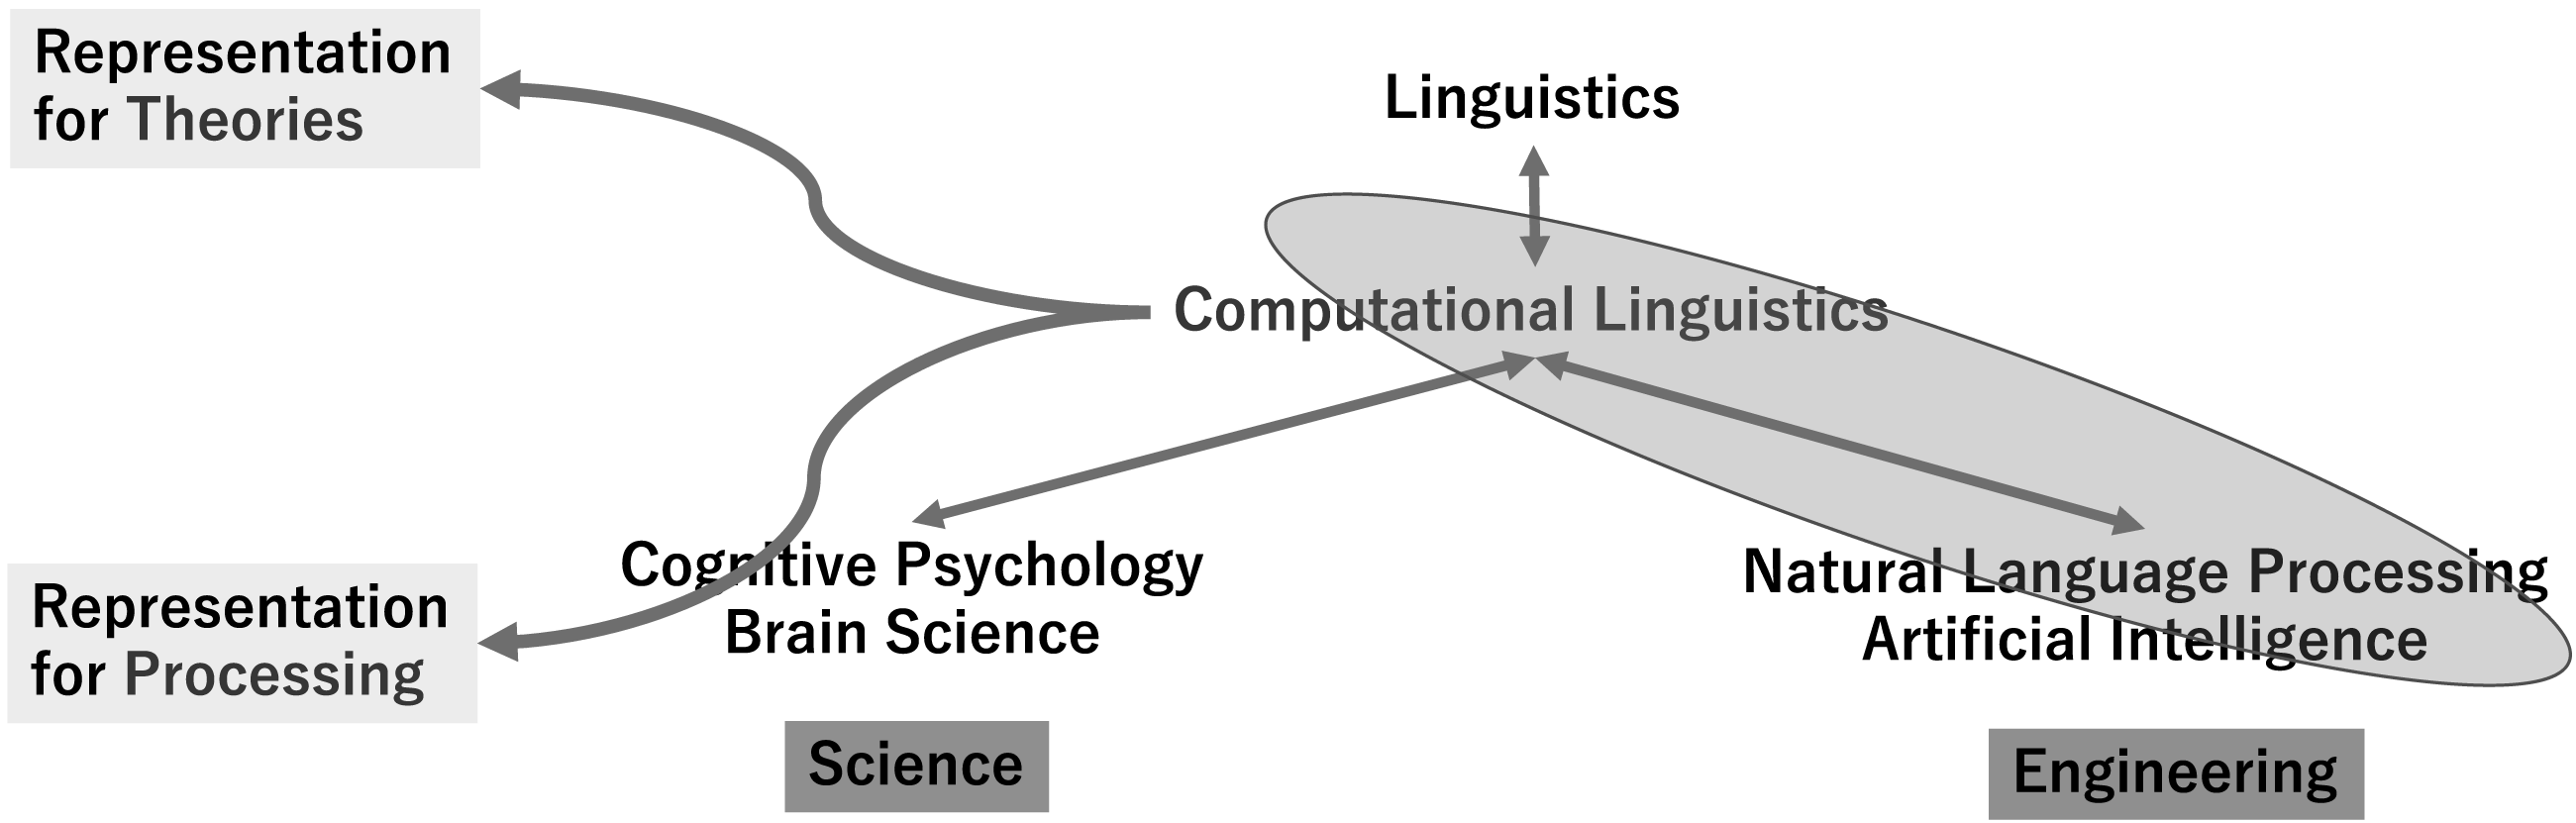
\includegraphics[width=14cm]{nlpcl}
\centering
\caption{Language-related disciplines \parencite{nlpandcl}}
\end{figure}
% }}}
  \section{Distributional semantics}
% {{{
The core idea behind distributional semantics has roots in American structuralism (Harris) and British lexicology (Firth) and is known as the distributional hypothesis. In its simplest form, it states that ``similarity in meaning results in similarity of linguistic distribution \parencite{harris}''.

The reverse of this statement is also true: ``the statistical distribution of linguistic items in context plays a key role in characterizing their semantic behavior \parencite{lenci}''. As a linguistics field, distributional semantics aims to learn the meanings of linguistics units from a corpus of text.

Distributional semantics was popularised by Firth in the 1950s. In a 1957 publication he wrote, ``the placing of a text as a constituent in a context of situation contributes to the statement of meaning since situations are set up to recognise use. <...> You shall know a word by the company it keeps! \parencite[11]{firth}''.

The ideas introduced by the distributional hypothesis have received attention in cognitive science \parencite{mcdonald} and language learning \parencite{yarlett}.
% }}}
        \paragraph{Overview}
% {{{
Distributional semantics has become widespread with the adoption of information technology in the field of linguistic research.

In its most frequent form, distributional semantics is applied by taking large amounts of text as input and producing a distributional model as output through the means of an abstraction algorithm \parencite{emerson}.

Distributional models rely on context to produce semantic representations. In other words, distributional models characterise the meanings of words through the context in which they have been observed \parencite{erkkatrin2}.

\begin{figure}[ht]% {{{
  \bigskip
  \begin{tikzpicture}[>={Classical TikZ Rightarrow[]}]
    \node[text width=6cm] at (0,11.5) {Planets of the solar system are orbiting the \textit{sun}. The \textit{moon} is orbiting the earth. It's his antique \textit{typewriter} clacking. <...>};
    \draw[line width=1pt, ->] (4.5,11.5) -- (5.5,11.5) node[pos=0.5,below=0.5cm]{algorithm};
    \node [shape=rectangle] at (10,11.5) {
      \ttfamily
      \begin{tabular}{|lcc|}
        \hline
        & dim1    & dim2    \\
        \hline
        sun      & 0.11023 & 0.53848 \\
        % \textbf{seli}    & 0.172305 & 0.824956 \\
        moon     & 0.21575 & 0.44034 \\
        % \textbf{lete}    & 0.280345 & 0.881492 \\
        typewriter & 0.52834 & 0.05389 \\
        % \textbf{mu}      & 0.370184 & 0.188725 \\
        \hline
      \end{tabular}
    };

    \draw[->, line width=1](0,0) -- (8,0) node[pos=0.5,below=1cm]{dim1};
    \draw[->, line width=1](0,0) -- (0,8) node[pos=0.58,rotate=90,left=1.5cm]{dim2};

    \foreach \x in {0,0.2,0.4,0.6}
        \draw (\x*10 cm,1pt) -- (\x*10 cm,-3pt)
            node[anchor=north] {$\x$};

    \foreach \y in {0,0.2,0.4,0.6}
        \draw (1pt,\y*10 cm) -- (-3pt,\y*10 cm)
            node[anchor=east] {$\y$};

    \draw[lightgray] (0, 0) grid[xstep=1, ystep=1] (8, 8);
    \foreach \Point/\PointLabel in {(1.1,5.3)/sun, (2.1,4.4)/{moon  (0.21575, 0.44034)}, (5.2, 0.5)/typewriter}
 % (6.7,1.2)/mu,
% (2.1,3.9)/mun, (2.8,4.8)/lete, (3.4, 6.8)/sewi, 
    \draw[draw=gray,fill=gray] \Point circle (0.08) node[above right] {$\PointLabel$};

    \node[draw, text width=10cm, fill=white] at (8, 2.5) {
      \ttfamily
      cosine\_similarity(sun, moon) = 0.9711
      cosine\_similarity(sun, typewriter) = 0.2959
    };

  \end{tikzpicture}
  \centering
  \caption{Distributional semantics, an illustrated overview}
\end{figure}% }}}

In a distributional model, the semantic representations are stored in the form of vectors. Vectors are lists of numbers that refer to points in a multi-dimensional space. These vectors are referred to as word vectors.

In the illustrated example, the model only has a dimensionality of two and thus can be mapped onto a two-dimensional plane without any further processing.

If this is not the case, the multi-dimensionality of the word vector encodings can be reduced to only two or three dimensions. Vectors that are relatively close in the multi-dimensional space are grouped into clusters, which are then retained in the low-dimensional space. The vectors can then be used to create a projection of the model which can be observed by the human eye.

All of the approaches to distributional semantics share the quality of learning semantic representations from a corpus in an unsupervised manner, without the involvement of humans.
% }}}
    \subsection{Distributional representations}
% {{{
Distributional representations are mathematic encodings of the distributional properties of words. Typically, in the form of a sequence of numbers. This sequence of numbers can be viewed as a multi-dimensional vector for the purposes of applying to them principles derived from liner algebra.

``Word vectors represent words as multidimensional continuous floating-point numbers where semantically similar words are mapped to proximate points in geometric space \parencite{ahireintro}''.

In simpler terms, a word vector is a numerical representation of a word in a corpus relative to every other word in that corpus.

``Vectors have geometrical interpretations: Vectors with n components define points (or arrows) in n-dimensional spaces. Therefore, distributional representations are geometrical representations of the lexicon in the form of a distributional vector space. The positions of lexemes in a distributional semantic space depend on their co-occurrences with linguistic contexts \parencite{lenci}''.
% }}}
      \subsubsection{Context types}
% {{{
Distributional representations output by a distributional model differ with respect to how the linguistic context is defined.

The contexts can be of the following types \parencite{lenci}:

\begin{itemize}
  \item \textbf{Undirected window-based collocate.} This context type includes words around the current word. No information as to whether the context words precede or follow after the current word is provided to the model. The window size typically ranges from 2 to 10.
  \item \textbf{Directed window-based collocate.} Unlike the previous context type, directed window-based contexts provide the direction in which the context word was seen relative to the current word.
  \item \textbf{Dependency-filtered syntactic collocate.} This context restricted the words which are analysed by the algorithm based on their syntactic roles. This information is however not provided to the model.
  \item \textbf{Dependency-typed syntactic collocate.} This context type provides the previously omitted syntactic type to the model.
  \item \textbf{Text region.} A text region context can represent any uniquely identifiable text sample: book chapters, web pages, or simply text portions of any fixed size.
\end{itemize}

The term window provides a physical analogy to a linguistic context. As the algorithm processes the corpus, the window of the context slides across the text, accounting for the words that can be seen through it.
% }}}
      \subsubsection{Semantic similarity metric}
% {{{
The semantic similarity between two vectors is primarily measured in two ways: using cosine similarity or the Euclidean distance.

The primary advantage of using one of these two methods is that they can be calculated for vectors of any dimensionality.

\paragraph{Euclidean distance}

The Euclidean distance between two points is the length of a line segment between the two points. It can also be defined as the shortest distance between two points in an n-dimensional space. For the purposes of calculating the Euclidean distance, the vectors are viewed as point coordinates \parencite{oduntan}.

\medskip
\[d_{Euc}(p, q) = \sqrt{\displaystyle\sum_{i=1}^{n} (p_i - q_i)^2} = \sqrt{(p_1 - q_1)^2 + (p_2 - q_2)^2 + ... + (p_n - q_n)^2}\]

\paragraph{Cosine similarity}

Cosine similarity is a measurement of similarity between two sequences of numbers. When calculating cosine similarity, the two sequences of numbers are viewed as vectors. Cosine similarity is equal to the cosine of the angle between two vectors, that is, the dot product of the vectors divided by the product of their lengths \parencite{oduntan}.

Cosine similarity always falls into the interval \([-1, 1]\). Two parallel vectors have a cosine similarity of \(1\), two orthogonal (perpendicular to each other) vectors have a cosine similarity of \(0\), while two opposite vectors have a cosine similarity of \(-1\).

\medskip
\[s_{cos}(A, B) := cos(\th) = \frac {A \cdot B}{||A|| \cdot ||B||} = \frac {\displaystyle\sum_{i=1}^{n} A_i B_i}{\sqrt{\displaystyle\sum_{i=1}^{n} A_i^2} \sqrt{\displaystyle\sum_{i=1}^{n} B_i^2}}\]
\medskip

This method was chosen to simplify the process of comparing similarities between vector pairs. Where the Euclidean distance provides an absolute value, the cosine similarity provides a fraction.
% }}}
    \subsection{Notable implementations}
      \subsubsection{Count vector model}
% {{{
The simplest implementations of distributional models feature counting algorithms. ``<...> these models record other words that have been observed in the vicinity of a target word in large text corpora, and form some sort of aggregate over the recorded context items. They then estimate the semantic similarity between words based on contextual similarity \parencite{erkkatrin2}''. These models are referred to as count models.

``Context items are counted only if they appear close to the target word, that is, if they are within the relevant context \parencite{erkkatrin2}''.

Count models operate on a window-based context. The window size is typically narrow (2-4 words). The window can be allowed to cross the boundaries of sentences or not \parencite{baroni}.
% }}}
      \subsubsection{Neural probabilistic language model}
% {{{
In recent years, the distributional model architecture has seen a notable shift to machine learning algorithms. With the improvements in hardware performance, the training of complex neural networks on corpora of larger sizes has become possible. 

The earlier machine learning-based models were plagued by the curse of dimensionality. This problem was solved in the model proposed by \parencite{bengio}. The proposed neural network model learns distributional representations and the generalisation function at the same time. The generalisation function is based on the estimates of the probability of a word appearing in the given context.

The architecture of this model ``consists of input, projection, hidden and output layers. At the input layer, \(N\) previous words are encoded using 1-of-\(V\) coding, where \(V\) is the size of the vocabulary. The input layer is then projected to a projection layer \(P\) that has dimensionality \(N \times D\), using a shared projection matrix. As only \(N\) inputs are active at any given time, composition of the projection layer is a relatively cheap operation \parencite{mikolov}''.

The training complexity of this model is

\[Q = N \times D + N \times D \times H + H \times V\]

where \(H\) is the size of the hidden layer.
% }}}
      \subsubsection{Recurrent neural net language model}
% {{{
This model architecture contains recurrent neural networks, meaning that as the model learns from the input, it produces output that is fed back into the model as input. The recurrent matrix connects hidden layers to itself using time-delayed connections. ``This allows the recurrent model to form some kind of short term memory, as information from the past can be represented by the hidden layer state that gets updated based on the current input and the state of the hidden layer in the previous time step \parencite{mikolov}''.

This model architecture consists of only input, hidden, and output layers, thus allowing for a reduction of complexity when compared to the neural probabilistic language model \parencite{mikolov}.

The training complexity of this model is

\[Q = H \times H + H \times V\]
% }}}
      \subsubsection{Continuous bag-of-words model}
% {{{
The first architecture of Word2vec proposed by Mikolov removes the non-linear hidden layer, further reducing complexity. The projection layer is shared for all words \parencite{mikolov}.

The continuous bag-of-words model is not influenced by history like the previous one. In a continuous bag-of-words model not only the words preceding the current word are used for context, but also the words that follow it.

This model attempts to predict the current word from the sum of the context vectors. This sum of vectors is referred to as a ``bag of words'', giving the name to the model. If the prediction of the word is correct after comparing it with the current word, its distributional representation is reinforced. If the prediction is wrong, the distributional representation is corrected.

The training complexity of this model is

\[Q = N \times D + D \times \log_2{V}\]

Because this model architecture produces the prediction as output, the learned weights of the hidden layer are what represents the word vectors.
% }}}
      \subsubsection{Continuous skip-gram model}
% {{{
The second architecture of Word2vec proposed by Mikolov has the opposite objective of the continuous bag-of-words model. The continuous skip-gram model predicts the surrounding context from the current word. Similar to the continuous bag-of-words model, when the continuous skip-gram model succeeds in predicting the context words, the semantic representation of the current word is reinforced. When it fails, it is corrected \parencite{mikolov}.

The training complexity of this model is

\[Q = N \times D + N \times D \times log_2{V} \]

While the complexity of this model is greater, the accuracy is also much greater \parencite{mikolov}. Similar to a continuous bag-of-words model, the weights of the hidden layer are the distributional representations.
% }}}
    \subsection{Applications}
% {{{
The data provided by the distributional model can be used directly to analyse the semantics of a language:

\begin{enumerate}
  \item \textbf{Semantic similarity.} By definition, distributional models provide data that quantifies semantic relatedness between individual words or expressions. This data can be interpreted by humans to draw conclusions about the meanings of words or used in other areas of natural language processing.
  \item \textbf{Word clustering.} Semantic representations tend to form groups in the multi-dimensional space. Word clustering refers to the ways and means by which these groups can be extracted as formal clusters \parencite{bekkerman}.
  \item \textbf{Automatic creation of thesauri.} The semantic similarity data can be further processed to produce lists of homonyms, synonyms, or even antonyms \parencite{henestroza}.
  \item \textbf{Word sense disambiguation.} This refers to a problem in computational linguistics that is concerned with identifying which sense of a word is used in a particular sentence \parencite{musto}.
  \item \textbf{Information retrieval.} Distributional models can be used to access semantically similar words to those of a query, expanding the retrieved results from exact word matching to semantically fuzzy matching \parencite{silva}.
  \item \textbf{Data mining.} In data mining, namely text mining, distributional models can provide means of identifying similar documents, thus narrowing the scope of a search \parencite[89]{dalianis}.
  \item \textbf{Paraphrasing.} The data provided by distributional models can supply paraphrasing algorithms with vocabulary, or aid in judging the relative semantic similarity between two paraphrases on a sentence level basis \parencite{desouki}.
  \item \textbf{Sentiment analysis.} Given a small list of words manually tagged with emotive potentials, distributional models can propagate these potentials through a corpus based on the semantic similarity between the tagged words \parencite{alshari}.
\end{enumerate}
% }}}
    \subsection{Curse of dimensionality}
% {{{
The curse of dimensionality refers to the phenomena that arise when organising data in high-dimensional spaces.

In the context of distributional models, dimensionality is determined by how many word relationships are accounted for each word by the model.

As the dimensionality of representations increases, the volume of the space they take up increases so fast that the available data becomes sparse. In other words, it becomes hard to make sense of the data as it becomes spread too thinly across the multi-dimensional space \parencite{venkat}.

A common solution to this is dimensionality reduction. ``Dimensionality reduction techniques transform dataset X with dimensionality D into a new dataset Y with dimensionality d, while retaining the geometry of the data as much as possible \parencite{sorzano}''.
% }}}
      \subsubsection{Principal component analysis}
% {{{
Principal component analysis aims to reduce the dimensionality of the distribution by finding a new set of variables that maximise variance and minimise information loss when compared to the original set of numbers. This is done through the process of determining the principal components and pushing the data towards them \parencite{richardson}.

The main limitation of principal component analysis is that it ``assumes a linear relationship between the features \parencite{hoz}'' of the items within the dataset. This causes it to struggle with classifying outliners.
% }}}
      \subsubsection{T-distributed stochastic neighbor embedding}
% {{{
T-distributed stochastic neighbor embedding reduces the dimensionality by examining the relative proximity between data points. In other words, it primarily attempts to preserve the local clusters present within the data as the dimensionality of the representation is reduced \parencite{van}.

This technique is better suited for working with data that does not lend itself well to principal components.
% }}}
  \section{Artificial languages}
% {{{
The term `artificial' is used to broadly refer to all languages that have been created through deliberate and conscious planning \parencite[41]{stria}. Under the broad umbrella of the term `artificial' reside predicate calculus and programming languages such as Lisp and C++.

``In the interlinguistic literature, the term `artificial', as opposed to `natural', is regarded as `crudely misleading' (Schubert 1989) because it suggests that languages created to facilitate international communication are in fact identical to machine or formulaic languages \parencite[45]{stria}''.

In an effort to avoid confusion with artificial languages of technical nature, the currently popular terms `constructed' and `invented' will be used throughout the rest of this paper.

It should be noted that the abbreviation `conlang' is also widely spread among the members of the community surrounding constructed languages.
% }}}
\subsection{The notion of a constructed language}
% {{{
Constructed languages are languages that have been purposely created to be similar or comparable in function to natural languages. The purpose behind the creation of constructed languages tends to vary greatly, ranging from the aim to create an auxiliary means of international communication, to artistic and philosophical expression.
% }}}
    \subsection{Notable constructed languages throughout history}
% {{{
``The dream of a perfect language did not only obsess European culture. The story of the confusion of tongues, and of the attempt to redeem its loss through the rediscovery or invention of a language common to all humanity, can be found in every culture \parencite[1]{eco}''.
% }}}
        \paragraph{Antiquity}
% {{{
The concept of a constructed language was first mentioned in writing by Athenaeus of Naucratis in his \textit{Deipnosophistae} (\textit{circa} \textsc{AD} 230). The languages he presented were not fully-fledged but of a rudimentary type known as a naming language. These languages were collections of neologisms that could be used to replace existing vocabulary or to refer to things that otherwise had no name. Athenaeus further writes of other people who invented their own words \parencite{sanders}.
% }}}
        \paragraph{Linguistic mysticism}
% {{{
Irish myths of the seventh century described the origin of Gaelic. According to \textit{Auraicept na n-Éces}, King Fénius Farsaid of Scythia travelled to the Tower of Babel after God fragmented human language. King Fénius and his many scholars studied the remains of the human language and combined its best fragments into a new and more perfect language, Gaelic \parencite{williams}.

The earliest attempt at language creation was Lingua Ignota by Hildegard of Bingen, a German Benedictine abbess and polymath, in the eleventh century. The underlying structure of the language was Latin, but the spelling was significantly altered. ``She did compose one macaronic antiphon, ``O orzchis Ecclesia,'' in which Latin and Lingua Ignota vocabulary alternate <...> Alternatively, if the Lingua had a second use as a secret language (possibly in the presence of outsiders) for Hildegard and her nuns, as some have suggested, this reviewer submits that verbs are not always needed for the achievement of communication: ``Enpholianz warinz nascutil'' (bishop / wart / nose) provides, if not exactly a sentence, an entirely understandable lexical string \parencite{higley}''.

``Hildegard also created Litteraæ Ignotæ 'unknown letters', a constructed writing system or \textit{neography}, which she used to represent Lingua Ignota \parencite{sanders}''. Despite the lack of grammatical depth in comparison to modern constructed languages, Lingua Ignota is widely praised as the first constructed language ever created.

From the belief in the connection between language creation and the divine arose the notion that languages inherited by humans from gods had become corrupted and now were causing confusion among the scholars and philosophers, impeding scientific progress. At the same time, by the 1600s, ``Latin, which was the sole language of education and the only language taught, experienced a decline, and there was no other language to replace it anytime soon \parencite[51]{stria}''. This caused a search for a new language to replace Latin and the subsequent creation of many philosophical constructed languages. These languages were centred around the idea of providing a top-down categorical view of the universe.

In his essay, Wilkins proposed one such universal philosophical language to replace Latin. This language was to be unambiguous and to encompass every concept in the universe, to overcome the curse of Babel \parencite[ch. 2, p. 1]{wilkins}.

Wilkins constructed a table of 40 major genera, which he then divided further into 251 characteristic differences. From them, he derived 2030 species, which appear in pairs. For example, ``starting from the major genus of Beasts, after having divided them into viviparous and oviparous, and after having subdivided the viviparous ones into whole footed, cloven footed and clawed, Wilkins arrives at the species Dog/Wolf \parencite[239]{eco}''.

Despite the initial acclaim and the interest it received from the king, the language soon fell into obscurity \parencite[25]{okrent}. This style of language creation continued into the seventeenth century and then was abandoned.
% }}}
        \paragraph{Early artistic languages}
% {{{
The sixteenth century also saw the beginning of artistic constructed languages. These languages ``are designed to suit a creative goal, usually as flavorful adornment in a work of fiction \parencite{sanders}''.

A prominent example of one of the earliest artistic constructed languages is the language of the fictional country Utopia (itself an invented word) from the 1516 novel by Sir Thomas More. The language was more than a naming language, though still mostly a relexification of Latin. It appears in the book only as a few isolated words in the text, as well as a four-line poem in the addendum written by More's friend Peter Giles \parencite{sanders}.

The main focus of constructed languages of this period was vocabulary, giving rise to many naming languages.
% }}}
        \paragraph{Early modern constructed languages}
% {{{
After a considerable decline of interest in philosophical languages, the efforts shifted towards a search for an idea auxiliarly language, which could be used as a lingua franca for people of different backgrounds.

The primary aim of the auxiliary constructed languages of this period was to become an international means of communication. Such languages are often referred to as international auxiliary languages.

One of the first fully-fledged auxiliary languages of this time was Jean Pirro's Univeralglot (1868), which is notable for incorporating linguistic features from multiple other languages. The other notable language was Johann Martin Schleyer's Volapük, the most successful auxiliary language until it was surpassed by Esperanto \parencite{sanders}.

Esperanto was created by Ludwik Lejzer Zamenhof in 1887 and remains the most widely spoken auxiliary constructed language. It still, however, fell short of Zamenhof's expectations.

``Volapük and Esperanto spurred the creation of many auxiliary languages, especially by those who sought to improve upon previous auxlangs. The first offshoot of Esperanto was Jacob Braakman's Mundolinco (1888), but the most successful was Ido, the result of a battle among Esperanto enthusiasts over whether Esperanto should be, or could even be allowed to be, improved \parencite{sanders}''. The modern critiques of Esperanto as an international auxiliary language note the irregularities of its grammar and the influences of Slavic languages on its design.

The artistic constructed languages of this time saw an increase in sophistication. The focus for still mainly on vocabulary, but the quantity and quality of the vocabulary have noticeably increased.
% }}}
        \paragraph{J. R. R. Tolkien}
% {{{
Tolkien saw language invention and myth-making as two interconnected forms of art. In a 1955 letter, Tolkien regarded his work as ``\textit{fundamentally} linguistic in inspiration \parencite[233]{letters}''.

In a 1958 letter to his son, Tolkien wrote about \textit{The Lord of the Rings}: ``Nobody believes me when I say that my long book is an attempt to create a world in which a form of language agreeable to my personal aesthetic might seem real. But it is true \parencite[285]{letters}''.

In a draft of a letter from 1967, Tolkien summed up his language invention: ``It must be emphasized that this process of invention was/is a private enterprise undertaken to give pleasure to myself by giving expression to my personal linguistic 'aesthetic' or taste and its fluctuations \parencite[411]{letters}''.

The constructed languages of the time reflected their intended practical use. Artistic languages were akin to flourishes added to a larger work of fiction, while auxiliary languages were conceived to support the full range of human communication. ``Tolkien bridged the gap between these two extremes by creating fully formed languages, but without any larger functionality or purpose beyond the sheer intellectual joy of doing so. However, he believed that his `secret vice` would not be taken seriously on its own, so he wrote his Middle-earth novels as a way to showcase them. Thus, while other writers created conlangs for their fiction, Tolkien created fiction for his conlangs \parencite{sanders}''.

Tolkien first revealed his love for language invention to the public in a 1931 essay entitled `A secret vice'. The essay concludes with poems in Qenya and a fragment in Noldorin (which later became known as Quenya and Sindarin), \parencite{tolkien83}.

Tolkien was a prolific language inventor. In his time, he created at least fifteen languages and dialects. His work did not stop merely at language creation but involved establishing both the detailed histories and the intricate interconnections between the languages of the Middle-earth. To an extent that Tolkien's `Tree of Tongues' was meant to reproduce an Indo-European genealogical tree model \parencite[101]{fimi}.

It is worth mentioning that within the lore of Middle-earth, the Black Speech was created by Sauron in mockery of the Elvish languages \parencite[20]{tolkien19}, ``to unite the forces of Mordor, making it one of the most notable examples of a conlang designed to be understood within its associated fictional setting as an actual conlang \parencite{sanders},'' rather than a natural language.
% }}}
        \paragraph{Modern constructed languages}
% {{{
Tolkien's work shaped the further history of constructed languages. Long viewed as a mere pastime, language invention has become a subject of academic study within linguistics.

From the 70s and well into the 2000s, the world saw the airing of many television series that featured constructed languages. Some of the most notable of them are \textit{Star Trek III: The Search for Spock} (1984, featuring Klingon) and \textit{Game of Thrones} (2011, featuring Dothraki).

``Aided by the expansion of the Internet in the 1990s, and especially the creation of the Conlang email list in 1991, modern conlangers have developed a robust community for exchanging ideas, critiques, and tools, allowing them to develop increasingly sophisticated and experimental conlangs \parencite{sanders}''.
% }}}
    \subsection{Classification}
      % stria fp.93, more proposed classifications of this nature
      \subsubsection{Traditional: structure and source material}
% {{{
The classification proposed by Couturat and Leau groups constructed languages based on their relationship with the source material or a lack thereof \parencite{couturat}:

\begin{itemize}
  \item \textbf{A priori.} Constructed languages that are not based on the elements of natural languages. ``A priori languages start from scratch with new symbols, signs or other elements devised to represent essential concepts \parencite{bianco}''.
  \item \textbf{A posteriori.} Constructed languages are based on the elements of natural languages. ``A posteriori languages draw their building blocks from existing languages  \parencite{bianco}''.
  \item \textbf{Mixed.} A combination of the two.
\end{itemize}

Several linguists have adopted this classification, most notably Janton, who provided several additions \parencite[5]{janton}:

\begin{enumerate}
  \item \textbf{A priori.} Metalanguages, schematic languages. These constructed languages are ``characterized by largely artificial, nonethnic word roots, schematic derivation, and fixed word categories (i.e., philosophical languages) \parencite[6]{janton}''.
  \item \textbf{A posteriori.} Naturalistic languages, pseudolanguages. ``These languages consciously imitate, in varying degrees, natural languages \parencite[5]{janton}''.
  \begin{itemize}
    \item \textbf{Minimal languages.} Simplified natural languages, living or dead.
    \item \textbf{Mixed languages.} Languages that use natural and non-natural roots.
      \begin{itemize}
        \item Languages that were schematically derived with natural word roots in distorted form (Volapük, 1880) or with both artistic and natural word roots (Perio, 1904).
        \item Languages that are partly schematic and partly naturalistic. Natural word roots in this group are rarely distorted (Esperanto, 1887).
      \end{itemize}
  \item \textbf{Naturalistic languages.}
    \begin{itemize}
      \item Languages with some schematic traits (Unial, 1903; Novial, 1928)
      \item Languages with natural derivation (Interlingua, 1940s).
    \end{itemize}
  \end{itemize}
\end{enumerate}

This classification presents a scale of artificiality, with languages derived from natural languages on one end and deliberately designed languages on the other. It is also primarily concerned with morphological and syntactic natures of derivation, not the intention with which the language was created.
% }}}
      \subsubsection{Traditional: purpose}
% {{{
``Another type of classification categorises artificial languages according to the purpose of creation \parencite[93]{stria}''. Kennaway provides the following division: universal languages (from a strive for perfection), international languages, languages of fiction, languages as recreation \parencite{kennaway}.

The primary concern with this way of classifying constructed languages this way lies in the fact that purpose is rarely binary. The prominent example are the languages which were constructed as recreation and later served as a tool in fictional worldbuilding.

\begin{figure}[ht]% {{{
  \bigskip
  \begin{tikzpicture}[>={Classical TikZ Rightarrow[]}]
    \draw[<->, line width=1](-4,0) -- (4,0)
      node[pos=0.0,left=0.5cm]{secret}
      node[pos=1.0,right=0.5cm]{public};
    \draw[<->, line width=1](0,-4) -- (0,4)
      node[pos=0.0,below=0.5cm]{fictional purposes}
      node[pos=1.0,above=0.5cm]{auxiliary purposes};
    \foreach \Point/\PointLabel in {
      (-3,-2.5)/Tolkien's,
      (3.5, 3.8)/Esperanto,
      (2.2, 2.8)/Interlingua,
      (2, -2.5)/Dothraki,
      (3.5, 1.5)/{Toki\ Pona}
    }
    \draw[draw=gray,fill=gray] \Point circle (0.08) node[above right] {$\PointLabel$};
  \end{tikzpicture}
  \centering
  \caption{Federico Gobbo's coordinate system}
\end{figure}% }}}

What followed were classifications that took a far more granular approach. ``A detailed typology is proposed by Albani and Buonarotti (1994), where a division is made into sacred and non-sacred languages. Sacred languages are further divided into structured (Bālaibalan) and non-structured with six subdivisions. Nonsacred languages split into languages with communicative and expressive goals both with further detailed subdivisions \parencite[93]{stria}''.

The classifications that followed saw a decrease in complexity and a shift to a more visual approach. Gobbo proposed a coordinate system which placed constructed languages between the "secret" and "public" extremes on the \textit{x axis} and "auxiliary purposes" and "fictional purposes" on the \textit{y axis} \parencite{gobbo}. This, however, is also not ideal, as the publicity of languages tends to shift greatly over time.

\begin{figure}[ht]% {{{
  \bigskip
  \begin{tikzpicture}[>={Classical TikZ Rightarrow[]}]
    \draw[line width=1](0,0) node[pos=0, left=0.8cm, below=0.2cm]{engelang} coordinate (a)--+(5,0) node[pos=1, right=0.8cm, below=0.2cm]{auxlang} coordinate (b)--+(60:5) node[pos=1, above=0.2cm]{artlang} coordinate (c) --cycle;
  \end{tikzpicture}
  \centering
  \caption{The modified Gnoli triangle}
\end{figure}% }}}

``One of the newest propositions widely spread on the Internet is the so-called Gnoli triangle. Claudio Gnoli, dissatisfied with the fact that his constructed language Liva was not easily classified, came up with an idea of a triangle whose vertices were labelled ‘artlang’ (artistic language), ‘auxlang’ (auxiliary language) and ‘loglang’ (logical language; the term ‘engelang’ was proposed later by And Rosta, apparently in 2001) \parencite[97]{stria}''.

Constructed languages placed on the Gnoli triangle can be characterised as a gradient between three distinct purposes, depending on where on the triangle they are located.

\begin{itemize}
  \item \textbf{Auxlang.} An international auxiliary language, that is, a language which was devised with the intention of being a means of international communication. The majority of international auxiliary languages are meant to be second languages and not to replace native languages \parencite{reed}.
  \item \textbf{Artlang.} A language created as a form of artistic expression or to fill an artistic role. Artistic languages often have irregular grammar systems, much like natural languages.
  \item \textbf{Engelang.} A language whose grammar or another feature is based on logic (a loglang) or a language which was created as an experiment or to prove a hypothesis of how languages function.
\end{itemize}
% }}}
      \subsubsection{Blanke's functional classification}
% {{{
The classification proposed by Blanke divides artificial languages into invented projects and fully-fledged languages \parencite{stria}:

\begin{itemize}
  \item \textbf{International auxiliary languages.} Languages intended to be used as a means of international communication.
  \item \textbf{Artistic languages.} Languages created for aesthetic reasons.
  \item \textbf{Constructed languages.} Languages invented to exercise the limits of language.
  \item \textbf{Exerimental languages.} Languages created to exercise a philosophical idea.
\end{itemize}
% }}}
        \bigskip
        \paragraph{Final note on classifications}
% {{{
Within the conlanging community, the terms from the above classifications are used by the principles of compositionality. Individual constructed languages are often described by having particular qualities borrowed from multiple classification systems.
% }}}
    \section{Summary}

This chapter discusses the following points related to the subjects of computational linguistics and constructed languages:

\paragraph{Distributional semantics}

\begin{itemize}
  \item The definition of computational linguistics, natural language processing, and distributional semantics.
  \item An overview of the main principles behind distributional semantics.
  \item A comparative evaluation of various distributional model implementations and their computational complexities.
  \item A comparison between two most widely used similarity metrics.
  \item A discussion of the primary problem of working with high-dimensional data, as well as widely used dimensionality reduction techniques.
\end{itemize}

\paragraph{Constructed languages}

\begin{itemize}
  \item The notion of a constructed language.
  \item A brief overview of the history of constructed languages.
  \item A number of approaches to classifying constructed languages.
\end{itemize}


\chapter{Language modelling and Toki Pona}
  \section{Toki Pona}
% {{{
Toki Pona is a philosophical artistic language created by Sonja Lang, a Canadian linguist and translator. The core vocabulary of Toki Pona consists of around 120 words and focuses on simple, near-universal concepts. Although Lang herself never planned the language as an international auxiliary language, it might indeed be considered as such \parencite[100]{stria}.

Lang has published two official books on Toki Pona. The first one, \textit{Toki Pona: The Language of Good} was published in May 2014 and is known as \textit{pu}. The second one, \textit{Toki Pona Dictionary} was published in July 2021 and is known as \textit{ku}.
% }}}
    \subsection{History}
      \subsubsection{Pre-pu}
% {{{
In the early days of Toki Pona, Lang experimented with both grammar and vocabulary. Numerous words from this period would be discarded before the online publication of the first draft of Toki Pona \parencite{evo}.

Lang first revealed the language to the public in a 2001 draft \parencite{firstdraft}. Multiple words are removed, replaced, and added. Toki Pona gains a small online following. The ``community primarily meets to discuss the language on Yahoo Groups, experimenting with and fleshing out the language \parencite{evo}''.

Around this time, Lang performs the first grammatical reform of Toki Pona. ``The words `en', `kin', `kan' and the concept of `and' have been relatively unstable and confusing in Toki Pona, as I have been experimenting to find the best system <...> There is no longer a way to divide between modifiers. This is no longer necessary. A `tall and good' person is simply a tall `good person' or a good `tall person', as you will. \parencite{enkinkan}''.

The community surrounding Toki Pona grows, as well as its corpus. This time sees the appearance of many early translations.

After more words are removed, for a while ``the total word count stabilises at 118 \parencite{evo}''.  ``The word \textit{pu} makes its first appearance but remains undefined until the publishing of \textit{Toki Pona: The Language of Good} \parencite{evo}''.

The preface of the book reads: ``Toki Pona is my philosophical attempt to understand the meaning of life in 120 words \parencite{pu}''. Lang continues to further outline the primary characteristics of the language:

\begin{itemize}
  \item ``Toki Pona is semantically, lexically, and phonetically minimalist''.
  \item ``In many ways, Toki Pona resembles a pidgin. When people from different cultures need to communicate, they must focus on the elements that are most universal to our human experience''.
  \item ``Toki Pona offers a path for semantic reduction. <...> we can distil our thoughts to their most fundamental units to discover what things really mean. We can understand complex ideas in terms of their smaller parts''.
  \item ``An inherent idea of goodness is transparent throughout the language.''
\end{itemize}
% }}}
      \subsubsection{Post-pu}
% {{{
After the publication of the first book, a few new words become official. Some portions of the grammar undergo significant changes, and many words receive new or altered definitions \parencite{evo}.

As the Toki Pona community rapidly grows, many idiolects permeate the way the language is spoken. Over a hundred new words is invented by the community. Most of them are relatively well adopted.

The first issue of the \textit{lipu tenpo} magazine is published online \parencite{liputenpo}. The second official Toki Pona book \textit{Toki Pona Dictionary} is published \parencite{ku}. Toki Pona is officially recognised by the ISO 639-3 registry under the code \textit{tok} \parencite{isoproof}.

The official Toki Pona subreddit sees an influx of members, reaching almost 11.000 subscribers at the time of writing. While no longer directly influencing the language, Lang remains an active member of the community.
% }}}

  \section{Distributional model}
    \subsection{Pre-processing}
% {{{
In the context of machine learning, noise contained within the input data is detrimental to the output. Before the data can be used as input, it has to be thoroughly cleaned from noise. This process is referred to as text pre-processing \parencite[49]{vajjala}.

The noise includes leftover formatting and HTML (HyperText Markup Language) tags, raw Unicode sequences, emojis, emoticons, punctuation, text in other languages, etc.

The Natural Language Toolkit Python library was used for the majority of text pre-processing tasks. ``NLTK is a leading platform for building Python programs to work with human language data \parencite{nltk}''.

Below is an example of a corpus entry at this stage:

\begin{lstlisting}
Pilin mi la, ni li pona: i<em>think</em> lon li lon is a goood way of saying c'est la vie :)  \n\n*also* TOKI!!! pan suwi &#xe339 li pona mute tawa mi a a a! :D &amp mi pali pona e pan suwi !! \n
\end{lstlisting}
% }}}
      \subsubsection{Tokenisation}
% {{{
Tokenisation is the process of splitting text into individual tokens, usually representing words and punctuation marks \parencite[49]{vajjala}.

Usually, this step is performed after the text has been split into sentences. The choice to perform tokenisation at this stage is supported by the fact that the source data contains an unusually large amount of text in other languages. Often, there is no separation between Toki Pona and other languages. If text tokenisation is performed first, it will prove easier to create custom rules for sentence segmentation at a later stage.

% After being tokenised, the example entry takes the shape of an array:
%
% \begin{lstlisting}
% ['Pilin', 'mi', 'la', ',', 'ni', 'li', 'pona', ':', 'i', '<', 'em', '>', 'think', '<', '/em', '>', 'lon', 'li', 'lon', 'is', 'a', 'goood', 'way', 'of', 'saying', "c'est", 'la', 'vie', ':', ')', '*', 'also', '*', 'TOKI', '!', '!', '!', 'pan', 'suwi', '&', '#', 'xe339', 'li', 'pona', 'mute', 'tawa', 'mi', 'a', 'a', 'a', '!', ':', 'D', '&', 'amp', 'mi', 'pali', 'pona', 'e', 'pan', 'suwi', '!', '!']
% \end{lstlisting}
% }}}
      \subsubsection{Noise removal}
% {{{
Every sequence that only contains symbols or a mixture of letters and symbols that is longer than one character is removed. The tokens which consist of only one punctuation mark are treated differently. Exclamation points and question marks are replaced with periods. The rest of the punctuation marks are removed

The tokens of the entry are then compared with a whitelist of allowed tokens. The whitelist includes all of the Toki Pona words, including the vocabulary that is not considered core vocabulary. When the matching is case-insensitive, meaning that it converts each token to lowercase before matching. The case is preserved.

The words which were not found to be in the Toki Pona vocabulary, are replaced with a period. The consecutive duplicate tokens which are not found in the whitelist are then removed from the sequence.

% After this is done, the entry looks like this:
%
% \begin{lstlisting}
% ['Pilin', 'mi', 'la', 'ni', 'li', 'pona', '.', 'lon', 'li', 'lon', '.', 'a', '.', 'la', '.', 'TOKI', '.', 'pan', 'suwi', 'li', 'pona', 'mute', 'tawa', 'mi', 'a', 'a', 'a', '.', 'mi', 'pali', 'pona', 'e', 'pan', 'suwi', '.']
% \end{lstlisting}
% }}}
      \subsubsection{Sentence segmentation}
% {{{
Sentence tokenisation is the process of splitting text based on the presence of punctuation marks \parencite[51]{vajjala}.

Because there are no punctuation marks left in the entry except for the periods, the entry can be split naively on them.

% \begin{lstlisting}
% [['Pilin', 'mi', 'la', 'ni', 'li', 'pona'], ['lon', 'li', 'lon'], ['a'], ['la'], ['TOKI'], ['pan', 'suwi', 'li', 'pona', 'mute', 'tawa', 'mi', 'a', 'a', 'a'], ['mi', 'pali', 'pona', 'e', 'pan', 'suwi']]
% \end{lstlisting}
% }}}
      \subsubsection{Normalisation}
% {{{
The first word of each sentence is brought to lowercase and compared with the whitelist. If there is a match, the word is replaced with its lowercase. The same is done for fully uppercase words in any part of the sentence.

The vocabulary of Toki Pona includes the word `ali', which is an alternative spelling of the word `ale'. Within the corpus, in all cases where `ali' appears, it is replaced with `ale'.

All of the proper names are removed from the corpus. All of the sentences shorter than three tokens are removed from the corpus as well.

The resulting entry takes the following shape:

\begin{lstlisting}
pilin mi la ni li pona
lon li lon
pan suwi li pona mute tawa mi a a a
mi pali pona e pan suwi
\end{lstlisting}
% }}}

    % TODO change link to wikipedia
    \subsection{Vector space model}
      \subsubsection{Training}
% {{{
The model is trained via the Gensim library. ``Gensim is an open-source library for unsupervised topic modelling and natural language processing, using modern statistical machine learning. \parencite{gensim}''. Gensim is chosen as it comes prepackaged with multiple distributional model architecture and a simple interface for training them.

Word2vec trains individual vectors for each word form. While this would be detrimental to training a model of a highly inflected language, no words in Toki Pona are ever inflected.

Before the model is trained, all low-frequency vocabulary is removed from the corpus. Consequently, sentences which are reduced to less than four words are removed as well. The vocabulary is kept to the set of words present in the original dictionary of the language.

The model is trained with the following parameters:

\begin{itemize}
  \item \textbf{Input.} 270903 (271K) sentences, 2239370 (2.2M) words total.
  \item \textbf{Window size.} 5 words.
  \item \textbf{Vector dimensionality.} 114 dimensions, to match the vocabulary size of the corpus.
\end{itemize}
% }}}
      \subsubsection{Dimensionality reduction}
% {{{
The Scikit-learn library is used to reduce the dimensionality of the model to two dimensions. Scikit-learn ``features various classification, regression and clustering algorithms including support-vector machines, random forests, gradient boosting, k-means and DBSCAN, and is designed to interoperate with the Python numerical and scientific libraries NumPy and SciPy \parencite{scikit}''.

Scikit-learn provides several methods for dimensionality reduction \parencite{tsne}. Among truncated singular value decomposition (Truncated SVD), principal component analysis (PCA), and t-distributed stochastic neighbour embedding (t-SNE) the best separation was achieved using t-SNE. Moreover, t-SNE ``takes a high dimensional data set and reduces it to a low dimensional graph that retains a lot of the original information \parencite{dimred}''.

The following parameters were used:

\begin{itemize}
  \item \textbf{Number of components.} 2, the dimensionality of the embedded space.
  \item \textbf{Perplexity or number of nearest neighbours.} 10, as no more than 10 words were expected to belong in the same semantic group.
  \item \textbf{Number of iterations.} 2500, for a higher degree of optimisation.
\end{itemize}
% }}}
      \subsubsection{K-means clustering}
% {{{

\begin{figure}[ht]% {{{
  \bigskip
  \begin{tikzpicture}[scale=0.045]
    \begin{scope}
      \clip (-170, -170) rectangle (210, 150);
      \draw[lightgray] (-500, -500) grid[xstep=20, ystep=20] (500, 500);
    \end{scope}
    \foreach \Point/\PointLabel/\Colo in {
      (-1.99,-27.58)/sama/34,
      (-102.6,-40.84)/nasin/16,
      (-108.03,-125.53)/sike/70,
      (-11.37,-52.37)/tan/46,
      (-119.69,-27.41)/kepeken/52,
      (-125.47,3.03)/nimi/16,
      (-127.39,12.73)/pu/16,
      (-143.63,-116.52)/wan/70,
      (-144.45,-133.36)/luka/70,
      (-15.71,-23.53)/lili/34,
      (-150.56,-123.77)/tu/70,
      (-156.04,-114.84)/nanpa/70,
      (-16.63,-81.64)/pilin/46,
      (-19.28,42.64)/pana/58,
      (-23.28,-13.83)/mute/40,
      (-27.19,20.31)/jo/58,
      (-29.25,-37.71)/ona/34,
      (-29.5,-58.17)/lawa/40,
      (-3.92,-96.7)/weka/46,
      (-31.34,-1.38)/kama/10,
      (-36.77,-17.58)/taso/10,
      (-38.46,-32.59)/mi/10,
      (-43.02,-50.94)/jan/22,
      (-44.08,33.71)/esun/58,
      (-44.53,44.8)/mani/58,
      (-47.87,5.46)/sin/16,
      (-47.99,106.82)/uta/64,
      (-49.09,-10.0)/ni/16,
      (-50.87,-67.04)/ale/22,
      (-53.25,18.4)/pali/16,
      (-58.67,-17.45)/pona/16,
      (-60.73,-49.2)/kulupu/16,
      (-62.14,-0.54)/ala/10,
      (-67.16,-28.94)/seme/16,
      (-68.3,102.37)/kute/52,
      (-69.58,-114.3)/open/28,
      (-7.69,-76.89)/ike/46,
      (-70.47,-8.29)/wile/16,
      (-72.61,47.81)/lukin/28,
      (-75.53,96.95)/musi/52,
      (-77.21,-108.26)/pini/28,
      (-78.22,9.0)/sina/16,
      (-79.08,110.8)/kalama/52,
      (-79.3,-130.08)/tenpo/28,
      (-79.34,-12.56)/ken/16,
      (-8.77,-3.88)/tawa/22,
      (-83.83,-49.42)/ijo/16,
      (-83.9,83.32)/ilo/52,
      (-84.8,-32.24)/ante/16,
      (-86.58,50.03)/sitelen/52,
      (-86.88,18.78)/anu/58,
      (-91.8,-117.79)/suno/28,
      (-95.93,47.91)/lipu/16,
      (-96.53,-127.01)/mun/70,
      (-98.38,-9.31)/sona/16,
      (-99.01,-21.74)/toki/16,
      (11.77,-43.15)/nasa/46,
      (113.5,17.01)/insa/58,
      (115.81,29.9)/selo/64,
      (118.49,52.76)/palisa/40,
      (119.44,42.33)/kiwen/64,
      (125.1,11.05)/poki/58,
      (128.95,-25.61)/kon/64,
      (129.82,-58.54)/pimeja/64,
      (13.16,7.89)/awen/82,
      (13.62,-71.54)/moli/76,
      (148.29,38.6)/walo/64,
      (149.66,-38.36)/lete/64,
      (150.71,-28.95)/seli/64,
      (157.36,70.82)/kule/40,
      (158.72,-16.5)/telo/64,
      (161.47,62.08)/laso/64,
      (164.97,40.21)/jelo/64,
      (166.25,20.75)/kasi/64,
      (167.44,49.91)/loje/64,
      (177.77,23.11)/kili/64,
      (179.06,-22.28)/ko/64,
      (18.3,-95.59)/sijelo/46,
      (180.11,-1.72)/moku/64,
      (186.86,-7.83)/suwi/64,
      (188.76,9.02)/pan/64,
      (23.59,-3.83)/poka/22,
      (23.99,124.68)/soweli/76,
      (25.01,17.09)/tomo/40,
      (26.33,-70.54)/utala/40,
      (28.83,114.46)/kala/76,
      (29.68,-40.05)/wawa/22,
      (36.51,108.0)/waso/76,
      (36.91,130.0)/akesi/76,
      (37.1,3.31)/ma/40,
      (4.48,-81.85)/pakala/46,
      (43.36,120.13)/pipi/76,
      (45.97,27.63)/meli/34,
      (47.63,-3.41)/suli/40,
      (5.03,88.39)/alasa/76,
      (5.43,22.77)/lape/82,
      (59.0,-17.91)/sewi/22,
      (61.15,-71.23)/mije/34,
      (62.62,-6.07)/anpa/22,
      (65.85,-54.5)/unpa/34,
      (66.88,12.01)/supa/82,
      (7.24,-1.58)/lon/28,
      (7.45,-109.57)/jaki/46,
      (71.76,-86.55)/mama/34,
      (74.41,28.67)/monsi/82,
      (75.11,-57.03)/olin/34,
      (75.25,-3.53)/noka/82,
      (79.68,48.74)/linja/76,
      (81.2,36.12)/sinpin/82,
      (9.62,122.35)/mu/76,
      (90.7,16.62)/lupa/28,
      (92.35,-13.35)/len/82,
      (98.3,38.36)/nena/40,
    }
    \draw[draw=black!\Colo,fill=black!\Colo] \Point circle (2.4) node[above] {\ttfamily\PointLabel};

  \end{tikzpicture}
  \centering
  \caption{Toki Pona vector space model in two-dimensional space}
\end{figure}% }}}

The primary objective of K-means clustering is to group similar data points in multi-dimensional space. These groups can then be assigned colours. The colours can then be used to draw the data points in any dimensionality, preserving the patterns.

The KMeansClusterer module from NLTK is used to achieve this. ``The K-means clusterer starts with k arbitrary chosen means then allocates each vector to the cluster with the closest mean. It then recalculates the means of each cluster as the centroid of the vectors in the cluster. This process repeats until the cluster memberships stabilise \parencite{kmeans}''.

The following parameters were used:

\begin{itemize}
  \item \textbf{Number of clusters.} 13, roughly 10 words in each cluster.
  \item \textbf{Distance.} Cosine distance.
\end{itemize}
% }}}
    \subsection{Observations}
% {{{
\begin{enumerate}
  \item The projection of the model is observed. The relative positions of words and their assigned clusters are noted down.
  \item For each analysed group, words are extracted from the projection as a semantic field based on their expected distribution.
  \item The semantic similarities between the words in the semantic field are calculated via cosine similarity from the perspective of the model, not the projection.
  \item The deviations of cosine similarity values returned by the model are correlated with the patterns of vocabulary use and dictionary definitions.
\end{enumerate}

    The cosine similarity between the vector of the \texttt{word_a} and the vector of the \texttt{word_b} is shown as \cs{word_a}{word_b}{cosine similarity}. Cosine similarity ranges from \([-1]\) to \([1]\).
% }}}
        \paragraph{Glossing abbreviations}
% {{{
The following abbreviations are used in the glosses below:

\begin{itemize}
  \item $cm$ -- context particle \tp{la}.
  \item $pm$ -- predicate particle \tp{li}.
  \item $do$ -- direct object particle \tp{e}.
  \item $em$ -- emotional emphasis particle \tp{a}.
  \item $im$ -- vocative imperative predicate particle \tp{o}.
\end{itemize}
% }}}
        \paragraph{kule}
% {{{
There are only five words in Toki Pona that can denote \tb{kule}{colors}: \tp{pimeja}, \tp{walo}, \tp{loje}, \tp{jelo}, \tp{laso}. For the rest of the colours, the rules of colour mixing apply: \textbf{jelo loje} can be used to mean \textit{orange}. Some of these words have broader meanings that describe not only the colour, but its vibrance, e.g \textbf{loje pimeja} can be used to mean \textit{dark red}.

\begin{figure}[ht]% {{{
  \def\angle{-45}
  \bigskip
  \begin{tikzpicture}[scale=0.046]
    \foreach \Point/\PointLabel/\Colo in {
      (157.36,70.82)/kule/40,
      (129.82,-58.54)/pimeja/64,
      (148.29,38.6)/walo/64,
      (164.97,40.21)/jelo/64,
      (167.44,49.91)/loje/64,
      (161.47,62.08)/laso/64,
      (-79.3,-130.08)/tenpo/28,
      (166.25,20.75)/kasi/64
    }
    \draw[draw=black!\Colo,fill=black!\Colo, rotate=\angle] \Point circle (2.4) node[above] {\ttfamily\PointLabel};
    \begin{scope}[on background layer]
      \clip ([shift={(-10,-10)}] current bounding box.south west) rectangle ([shift={(10, 10)}] current bounding box.north east);
      \draw[lightgray, rotate=\angle] (-500, -500) grid[xstep=20, ystep=20] (500, 500);
    \end{scope}
  \end{tikzpicture}
  \centering
  \caption{kule, \(\angle\textdegree\)}
\end{figure}% }}}

The presence of \tp{kasi} among the colours can be attributed to Toki Pona having only one word for blue and green -- \textbf{laso}. Despite the existence of many languages that also have one word for blue and green, the distribution is related the fact that many Toki Pona speakers opt to refer to the colour green unambiguously \cs{kasi}{kule}{0.51}.

The word \textbf{pimeja} is considerably separated from the rest of the colours. This is explained by it often appearing near \tp{tenpo}. In turn, \textbf{tenpo pimeja} is a common way of referring to \textit{nighttime}:

\begin{exe}
  \ex
  \gll tenpo pimeja la, mi lape. \\
       time black $cm$ I sleep \\
  \glt I sleep at night.
\end{exe}

Among words for colours, this property is unique to \textbf{pimeja}: \cs{walo}{tenpo}{-0.03}, \cs{loje}{tenpo}{-0.07}, \cs{jelo}{tenpo}{-0.11}, \cs{laso}{tenpo}{-0.06}. Interestingly, \textbf{pimeja} experiences an even semantic split between \textbf{kule} and \textbf{tenpo}: \cs{pimeja}{kule}{0.24}, \cs{pimeja}{tenpo}{0.24}.
% }}}
        \paragraph{nanpa}
% {{{
There are a number of words which are related to \textbf{nanpa} (numerals) in the vocabulary of Toki Pona: \tp{wan} used to mean \textit{one}, \tp{tu} used to mean \textit{two}, \tp{luka} used to mean \textit{five}, \tp{ale} used to mean \textit{one hundred}, \tp{ala} used to mean \textit{zero}, and \tp{mute}.

\begin{figure}[ht]% {{{
  \def\angle{-45}
  \bigskip
  \begin{tikzpicture}[scale=0.046]
    \begin{scope}[rotate=\angle]
      \foreach \Point/\PointLabel/\Colo in {
        (-156.04,-114.84)/nanpa/70,
        (-143.63,-116.52)/wan/70,
        (-23.28,-13.83)/mute/40,
        (-150.56,-123.77)/tu/70,
        (-50.87,-67.04)/ale/22,
        (-62.14,-0.54)/ala/10,
        (-144.45,-133.36)/luka/70
      }
      \draw[draw=black!\Colo,fill=black!\Colo] \Point circle (2.4) node[above] {\ttfamily\PointLabel};
    \end{scope}
    \begin{scope}[on background layer]
      \clip ([shift={(-10,-10)}] current bounding box.south west) rectangle ([shift={(10, 10)}] current bounding box.north east);
      \draw[lightgray, rotate=\angle] (-500, -500) grid[xstep=20, ystep=20] (500, 500);
    \end{scope}
  \end{tikzpicture}
  \centering
  \caption{nanpa, \(\angle\textdegree\)}
\end{figure}% }}}

The word \textbf{luka} is semantically detached from its lower body counterpart, \tp{noka}: \cs{luka}{noka}{0.35}, \cs{luka}{nanpa}{0.76}. This highlights the unique ability of \textbf{luka} to denote numerals among other words that indicate parts of the body.

Despite one of the word sense of \textbf{mute} being \textit{quantity}, it experiences little semantic similarity with \textbf{nanpa}: \cs{mute}{nanpa}{0.25}, as \textbf{mute} is most commonly used for specifying \textit{intensity}:

\begin{exe}
  \ex
  \gll mi pilin pona mute a. \\
       I feel good very $em$ \\
  \glt I am feeling very good!
\end{exe}

The position of \textbf{ale} and \textbf{ala} are exlained by their more frequent usage as a pronouns and a negation particle in the case of \textbf{ala}.

One of the secondary uses of \textbf{nanpa} and \textbf{wan} is involved in expressing high degree of positivity towards something:

\begin{exe}
  \ex
  \gll kili ma li pona nanpa wan. \\
       vegetable land $pm$ good number one \\
  \glt Potatoes are the best.
\end{exe}

The distribution shows that this use of \textbf{nanpa wan} is farily uncommon: \cs{[nanpa, wan]}{[pona, mute]}{0.14}.
% }}}
        \paragraph{soweli}
% {{{
% TODO alasa-soweli?
The cluster \tp{soweli} contains words that refer to the members of the animal kingdom: \tp{akesi}, \tp{kala}, \tp{waso}, \tp{pipi}.

\begin{figure}[ht]% {{{
  \def\angle{-45}
  \bigskip
  \begin{tikzpicture}[scale=0.046]
    \begin{scope}[rotate=\angle]
      \foreach \Point/\PointLabel/\Colo in {
        (23.99,124.68)/soweli/76,
        (28.83,114.46)/kala/76,
        (36.51,108.0)/waso/76,
        (43.36,120.13)/pipi/76,
        (36.91,130.0)/akesi/76,
        (9.62,122.35)/mu/76,
        (5.03,88.39)/alasa/76,
        (-44.53,44.8)/mani/58
      }
      \draw[draw=black!\Colo,fill=black!\Colo] \Point circle (2.4) node[above] {\ttfamily\PointLabel};
    \end{scope}
    \begin{scope}[on background layer]
      \clip ([shift={(-10,-10)}] current bounding box.south west) rectangle ([shift={(10, 10)}] current bounding box.north east);
      \draw[lightgray, rotate=\angle] (-500, -500) grid[xstep=20, ystep=20] (500, 500);
    \end{scope}
  \end{tikzpicture}
  \centering
  \caption{soweli, \(\angle\textdegree\)}
\end{figure}% }}}

The onomatopoeia \tp{mu} is also present in this cluster: \cs{soweli}{mu}{0.54}. Among other words in the cluster, \textbf{pipi} is the least semantically related to \textbf{mu} by a substantial margin: \cs{pipi}{mu}{0.29}. This is perhaps related to the fact that \textit{bugs} do not produce sound with their mouths.

The dictionary entry for \textbf{akesi} contains the now considered outdated \textit{non-cute animal} word sense. The fact that this definition was in use at a time is evident from the semantic similarity between \tp{suwi} and \textbf{akesi}: \cs{akesi}{suwi}{0.27}; compared to the other members of the cluster: \cs{soweli}{suwi}{0.53}, \cs{kala}{suwi}{0.51}, \cs{waso}{suwi}{0.49}, \cs{pipi}{suwi}{0.45}. Also, \textbf{akesi} is the most semantically related to \tp{ike} among other words to animals.

The word \tp{mani} has the secondary definition of a \textit{large domesticated animal}. This could be attributed to the themes of hunter-gatherer culture that permeate the language. In the model, only a very weak semantic connection between \textbf{mani} and \textbf{soweli} is present: \cs{mani}{soweli}{0.18}.

Keeping with the theme of hunter-gatherer culture, \tp{alasa} is also in the proximity of the cluster, despite sometimes being used as a pre-verb to mean \textit{to try to}. The closest pair within the cluster is \cs{alasa}{kala}{0.56}, used to mean \textit{fishing}. The connection between \tp{kili} and \textbf{alasa} is also present: \cs{alasa}{kili}{0.14}, albeit a much weaker one.
% }}}
        \paragraph{kalama}
% {{{
A small cluster of \tp{kalama} includes words related to sound production and perception: \tp{uta}, \tp{kute}. The earlier discussed \textbf{mu} is also in the vicinity of this cluster: \cs{mu}{kalama}{0.3}.

\begin{figure}[ht]% {{{
  \def\angle{135}
  \bigskip
  \begin{tikzpicture}[scale=0.046]
    \begin{scope}[rotate=\angle]
      \foreach \Point/\PointLabel/\Colo in {
        (-79.08,110.8)/kalama/52,
        (-75.53,96.95)/musi/52,
        (-47.99,106.82)/uta/64,
        (9.62,122.35)/mu/76,
        (-68.3,102.37)/kute/52
      }
      \draw[draw=black!\Colo,fill=black!\Colo] \Point circle (2.4) node[above] {\ttfamily\PointLabel};
    \end{scope}
    \begin{scope}[on background layer]
      \clip ([shift={(-10,-10)}] current bounding box.south west) rectangle ([shift={(10, 10)}] current bounding box.north east);
      \draw[lightgray, rotate=\angle] (-500, -500) grid[xstep=20, ystep=20] (500, 500);
    \end{scope}
  \end{tikzpicture}
  \centering
  \caption{kalama, \(\angle\textdegree\)}
\end{figure}% }}}

The presense of \tp{musi} in the cluster is expected due to \textit{music} being often described as \textbf{kalama musi}:

\begin{exe}
  \ex
  \gll mi kute e kalama musi la, mi wile tawa musi. \\
       I hear $do$ sound entertaining $cm$ I want move entertainingly. \\
  \glt Listening to music makes me want to dance.
\end{exe}

Music is among the most universal forms of entertainment that are discussed online, and the semantic distribution is the evidence of that. The semantic similarity between the two words is \cs{kalama}{musi}{0.66}.
% }}}
        \paragraph{selo}
% {{{
There are multiple words in Toki Pona whose primary or secondary purpose is related to describing the general \textbf{selo} (shape) of an object. The cluster primarily includes words which refer to parts of the body: \tp{linja}, \tp{nena}, \tp{selo}.

While not immediately recognisable by the dictionary entry, \tp{kiwen} can be used to refer to \textit{teeth} as \textbf{kiwen uta}, \tp{uta}: \cs{kiwen}{uta}{0.47}.

Likewise, the word \tp{palisa} can be combined with \tp{sijelo} to refer to \textit{bones}, albeit the distribution shows that it is a less frequent pattern \cs{palisa}{sijelo}{0.24}.

\begin{figure}[ht]% {{{
  \def\angle{-35}
  \bigskip
  \begin{tikzpicture}[scale=0.046]
    \begin{scope}[rotate=\angle]
      \foreach \Point/\PointLabel/\Colo in {
        (-95.93,47.91)/lipu/16,
        (115.81,29.9)/selo/64,
        (125.1,11.05)/poki/58,
        (-108.03,-125.53)/sike/70,
        (118.49,52.76)/palisa/40,
        (119.44,42.33)/kiwen/64,
        (79.68,48.74)/linja/76,
        (98.3,38.36)/nena/40
      }
      \draw[draw=black!\Colo,fill=black!\Colo] \Point circle (2.4) node[above] {\ttfamily\PointLabel};
    \end{scope}
    \begin{scope}[on background layer]
      \clip ([shift={(-10,-10)}] current bounding box.south west) rectangle ([shift={(10, 10)}] current bounding box.north east);
      \draw[lightgray, rotate=\angle] (-500, -500) grid[xstep=20, ystep=20] (500, 500);
    \end{scope}
  \end{tikzpicture}
  \centering
  \caption{selo, \(\angle\textdegree\)}
\end{figure}% }}}

The word sense of \tp{lipu} signifying a \textit{flat object} is overshadowed by the word sense \textit{book}. The semantic similarity between \textbf{lipu} and \textbf{palisa} is \cs{lipu}{palisa}{0.0}.

The position of \tp{sike} is explained by it primarily being used to describe time \cs{sike}{tenpo}{0.43}:

\begin{exe}
  \ex
  \gll suno sike sina o pona a! \\
       sun round you $im$ good $em$ \\
  \glt Have a Happy New Year!
\end{exe}
% }}}
        \paragraph{moku}
% {{{
The \tp{moku} cluster includes the following words: \tp{pan}, \tp{kili}, \tp{telo}, as well as \tp{suwi}.

\begin{figure}[ht]% {{{
  \def\angle{-45}
  \bigskip
  \begin{tikzpicture}[scale=0.046]
    \begin{scope}[rotate=\angle]
      \foreach \Point/\PointLabel/\Colo in {
(158.72,-16.5)/telo/64,
(150.71,-28.95)/seli/64,
(149.66,-38.36)/lete/64,
(177.77,23.11)/kili/64,
(188.76,9.02)/pan/64,
(180.11,-1.72)/moku/64,
(186.86,-7.83)/suwi/64,
(148.29,38.6)/walo/64
      }
      \draw[draw=black!\Colo,fill=black!\Colo] \Point circle (2.4) node[above] {\ttfamily\PointLabel};
    \end{scope}
    \begin{scope}[on background layer]
      \clip ([shift={(-10,-10)}] current bounding box.south west) rectangle ([shift={(10, 10)}] current bounding box.north east);
      \draw[lightgray, rotate=\angle] (-500, -500) grid[xstep=20, ystep=20] (500, 500);
    \end{scope}
  \end{tikzpicture}
  \centering
  \caption{moku, \(\angle\textdegree\)}
\end{figure}% }}}

The position of \textbf{suwi} in the distribution hints at it commonly being used to specify taste: \cs{suwi}{moku}{0.67}. The word sense \textit{cute} is hovewer also popular, as the semantic similarity between \textbf{suwi} and \textbf{soweli} is \cs{suwi}{soweli}{0.53}. The most \textbf{suwi} food related word is \textbf{pan}, as \textbf{pan suwi} is a common way of referring to \textit{sweet backed goods}.

The semantic similarity between \textbf{moku} and \tp{ko} is \cs{moku}{ko}{0.54}, suggesting that \textbf{ko} is commonly used to describe food, from \textit{sauces} to \textit{cheeses}.

The words \textbf{telo} and \tp{walo} are also closely related: \cs{telo}{walo}{0.64}, as \textbf{telo walo} is a common way of referring to \textit{milk}.

The word \tp{seli} is more semantically related to \textbf{telo} than \tp{telo}: \cs{telo}{seli}{0.67}, \cs{telo}{lete}{0.53}, suggesting that \textbf{seli} is used to describe the process of \textit{cooking}.
% }}}
        \paragraph{ike}
% {{{
The vocabulary cluster \tp{ike} mainly consists of words that are percieved as something \textit{bad}: \tp{pakala}, \tp{moli}, \tp{utala}, \tp{jaki}, as well as \tp{weka}.

\begin{figure}[ht]% {{{
  \def\angle{-10}
  \bigskip
  \begin{tikzpicture}[scale=0.046]
    \begin{scope}[rotate=\angle]
      \foreach \Point/\PointLabel/\Colo in {
        (-16.63,-81.64)/pilin/46,
        (4.48,-81.85)/pakala/46,
        (18.3,-95.59)/sijelo/46,
        (7.45,-109.57)/jaki/46,
        (-3.92,-96.7)/weka/46,
        (26.33,-70.54)/utala/40,
        (-29.5,-58.17)/lawa/40,
        (13.62,-71.54)/moli/76
      }
      \draw[draw=black!\Colo,fill=black!\Colo] \Point circle (2.4) node[above] {\ttfamily\PointLabel};
    \end{scope}
    \begin{scope}[on background layer]
      \clip ([shift={(-10,-10)}] current bounding box.south west) rectangle ([shift={(10, 10)}] current bounding box.north east);
      \draw[lightgray, rotate=\angle] (-500, -500) grid[xstep=20, ystep=20] (500, 500);
    \end{scope}
  \end{tikzpicture}
  \centering
  \caption{ike, \(\angle\textdegree\)}
\end{figure}% }}}

The presence of \tp{sijelo} and \tp{pilin} in the cluster can be explained by them often appearing in sentences related to injury, sickness, or general physical state:

\begin{exe}
  \ex
  \gll sijelo mi li pilin ike. \\
       body I $pm$ feel bad $em$ \\
  \glt I'm not feeling well.
\end{exe}

The proximity of \tp{lawa} to the cluster may be related to negative undertones surrounding the idea of \textit{control}: \cs{lawa}{pona}{0.0}, \cs{lawa}{ike}{0.23}, where \tp{pona} is the antonym of \textbf{ike}.
% }}}
        \paragraph{nimi sama ijo}
% {{{
The cluster of \textbf{nimi sama ijo} or pronouns includes the words \tp{mi}, \tp{sina}, \tp{ona}. The words \tp{ni}, \tp{ale}, and \tp{ala}.

\begin{figure}[ht]% {{{
  \def\angle{-135}
  \bigskip
  \begin{tikzpicture}[scale=0.046]
    \begin{scope}[rotate=\angle]
      \foreach \Point/\PointLabel/\Colo in {
(-38.46,-32.59)/mi/10,
(-78.22,9.0)/sina/16,
(-29.25,-37.71)/ona/34,
(-49.09,-10.0)/ni/16,
(-43.02,-50.94)/jan/22,
(-62.14,-0.54)/ala/10,
(-50.87,-67.04)/ale/22
      }
      \draw[draw=black!\Colo,fill=black!\Colo] \Point circle (2.4) node[above] {\ttfamily\PointLabel};
    \end{scope}
    \begin{scope}[on background layer]
      \clip ([shift={(-10,-10)}] current bounding box.south west) rectangle ([shift={(10, 10)}] current bounding box.north east);
      \draw[lightgray, rotate=\angle] (-500, -500) grid[xstep=20, ystep=20] (500, 500);
    \end{scope}
  \end{tikzpicture}
  \centering
  \caption{ike, \(\angle\textdegree\)}
\end{figure}% }}}

Interestingly, \tp{jan} is also part of this cluster. Syntactically, proper nouns behave like adjectives in Toki Pona. This explaines the semantic similarity between \textbf{jan} and \textbf{ona}: \cs{jan}{ona}{0.53}. In fact, they are the closest neighbors within the model.
% }}}
      \paragraph{tenpo}
% {{{
The words from the \textbf{nanpa} cluster are often used to quantify time. The numerals are listed in the descending order of magnitude and are added together:

\begin{exe}
  \ex
  \gll tenpo suno pini luka tu la, mi lukin e sitelen tawa ni. \\
       time sun finished five two $cm$ I look $do$ picture moving this \\
  \glt I watched this movie a week ago.
\end{exe}

This explains the high degree of semantic relatedness between the words that belong to these two clusters. Moreover, \textbf{tenpo wan} is sometimes used to mean \textit{once}.

\begin{figure}[ht]% {{{
  \def\angle{-22.5}
  \bigskip
  \begin{tikzpicture}[scale=0.046]
    \begin{scope}[rotate=\angle]
      \foreach \Point/\PointLabel/\Colo in {
        (-77.21,-108.26)/pini/28,
        (-69.58,-114.3)/open/28,
        (-91.8,-117.79)/suno/28,
        (-108.03,-125.53)/sike/70,
        (-96.53,-127.01)/mun/70,
        (-79.3,-130.08)/tenpo/28,
        (-15.71,-23.53)/lili/34,
        (47.63,-3.41)/suli/40,
        (-23.28,-13.83)/mute/40,
        (23.59,-3.83)/poka/22,
        (129.82,-58.54)/pimeja/64,
        (-156.04,-114.84)/nanpa/70,
        (-150.56,-123.77)/tu/70,
        (-143.63,-116.52)/wan/70,
        (-144.45,-133.36)/luka/70,
        (-31.34,-1.38)/kama/10
      }
      \draw[draw=black!\Colo,fill=black!\Colo] \Point circle (2.4) node[above] {\ttfamily\PointLabel};
    \end{scope}
    \begin{scope}[on background layer]
      \clip ([shift={(-10,-10)}] current bounding box.south west) rectangle ([shift={(10, 10)}] current bounding box.north east);
      \draw[lightgray, rotate=\angle] (-500, -500) grid[xstep=20, ystep=20] (500, 500);
    \end{scope}
  \end{tikzpicture}
  \centering
  \caption{tenpo, \(\angle\textdegree\)}
\end{figure}% }}}

In terms of \textbf{tenpo}, the words \tp{pini} and \tp{kama} are antonyms used to refer to the \textit{past} and \textit{future} time respectively. Similar contexts hint at their semantic relatedness: \cs{pini}{kama}{0.47}. The words \textbf{pini} and \textbf{open} are higly related due to their usage of pre-verbs to mean \textit{finish} and \textit{begin doing something} respectively: \cs{pini}{open}{0.67}, \textbf{tenpo open} can mean \textit{in the beginning} as well.

As was discussed earlier, \tp{sike} refers to a \textit{season} or a \textit{year} in the context of time.

The word \tp{suno} is also highly temporal due to being used to describe \textit{days} or \textit{daytime}: \cs{tenpo}{suno}{0.56}. Its counterpart \tp{mun} refers to a \textit{month} in the context of time: \cs{tenpo}{mun}{0.59}.

The words \tp{mute} and \tp{lili} are used to quantify frequency or infrequency of repeated actions in the specified time.

Sometimes, \tp{poka} is used to specify time not too far removed from the present: \cs{tenpo}{poka}{0.26}.
% }}}
      \paragraph{mama}
% {{{
The word cluster centered around \tp{mama} includes words related to the concept of family: \tp{meli}, \tp{mije}, \tp{unpa}, \tp{olin}, \tp{sama}, \tp{lili}.

The presense of \textbf{lili} is explained by \textbf{jan lili} being a common way to refer to a \textit{child}: \cs{mama}{lili}{0.34}.
% }}}
      \paragraph{esun}
% {{{
The small cluster centered around \tp{esun} represents words that are related to the idea of \textit{commerce}: \tp{mani}, \tp{pali}, \tp{jo}, \tp{moku}.
% }}}

  \section{Summary}

This chapter provides a short history of Toki Pona, as well as the following steps of the applied research:

\begin{itemize}
  \item The pre-processing, tokenisation, noise removal, sentence segmentation, and normalisation of textual corpora.
  \item The details of how the distributional model of Toki Pona was constructed: the notes on the training process, dimensionality reduction, and K-means clustering.
  \item A detailed analysis of the vocabulary of Toki Pona based on the data obtain via the constructed distributional model.
\end{itemize}

All of the objectives set in the introduction of this research were achieved in the course of this chapter.

\chapter{Conclusion}
% {{{
The small size of the Toki Pona vocabulary and the low precision of word definitions encourage the use of semantic decomposition when speaking about concepts of higher degrees of complexity. While this feature of the language broadens the range of contexts in which a particular word can appear, certain patterns within the vocabulary were found to be clearly defined.

The use of the principles behind distributional semantics in a semantic analysis of a language remains a novel approach. The results greatly depend one the size of the available corpora and the lexical and morphological complexity of the language being analysed. In the case of Toki Pona, which is neither inflected nor contains a large number of lexemes, it has proven to be an extremely effective means of analysing word senses of individual vocabulary items.

The analysis showed that Toki Pona substantially differs from the language which was originally published back in 2014. Some word senses have largely fallen out of use, some asserted dominance over others. With the help of the distributional model created in the course of this research, predominant word senses were separated from secondary ones.

The scope of the analysis did not only involve discerning word senses, but delved into the subject of attributing words to the conversational contexts in which these words tend to appear in. Through this processes, certain obscure relationships between word pairs were brought to light.

The author hopes that this research will serve as the groundwork for further academic studies into the semantics of conlangs; and, of course, Toki Pona, one truly fascinating language.
% }}}
\smallskip

\vspace*{\fill}
  \begin{minipage}{0.69\textwidth}
    \newfontfamily\myfont{linja pona 4.9}
    \myfont\Large
    \setlength\parindent{0cm}
    \def\baselinestretch{1.15}\selectfont

    toki a

    \bigskip

    sina ken toki kepeken toki+pona la sina sona e ijo mute pi lipu ni

    \bigskip

    lipu ni li pali suli pi sona musi mi. lipu ni la mi toki e nimi sona suli e ijo ante mute e pilin mi. ni li tan ni: jan suli pi pana sona la mi awen e lipu sona mi

    \bigskip

    wile mi la sina o pilin ike ala tan nasin sona mi. toki+pona li pona mute tawa mi. tan ni la mi wile lukin sona e toki+pona

    \bigskip

    sina lukin e lipu ni la o pona tawa sina. o pona mute tawa mama pi toki+pona a

    \bigskip

    o pona tawa meli mi. mi toki mute e toki+pona la ona li pilin lape. taso ona li kama sona e toki+pona lili

    \bigskip

    ni ale li pini la o pona tawa kijetesantakalu a

  \end{minipage}
\vspace*{\fill}








\printbibliography[heading=bibintoc, title={References}, nottype=online]
\printbibliography[heading=bibintoc, title={Online resources}, type=online]

\chapter{Supplementary marterial}
  \section{Model vectors}
The two-dimensional projection of the semantic model constructed in the course of this reseach.
% {{{
\begin{longtable}{lcclcc}
  \textbf{word} & \textbf{x} & \textbf{y} & \textbf{word} & \textbf{x} & \textbf{y} \\
  \endfirsthead
  \multicolumn{6}{c}{\tablename~\thetable: Toki Pona model projection} \\[0.25cm]
  \textbf{word} & \textbf{x} & \textbf{y} & \textbf{word} & \textbf{x} & \textbf{y} \\
  \endhead
akesi & 36.91 & 130.0 & ala & -62.14 & -0.54 \\
alasa & 5.03 & 88.39 & ale & -50.87 & -67.04 \\
anpa & 62.62 & -6.07 & ante & -84.8 & -32.24 \\
anu & -86.88 & 18.78 & awen & 13.16 & 7.89 \\
esun & -44.08 & 33.71 & ijo & -83.83 & -49.42 \\
ike & -7.69 & -76.89 & ilo & -83.9 & 83.32 \\
insa & 113.5 & 17.01 & jaki & 7.45 & -109.57 \\
jan & -43.02 & -50.94 & jelo & 164.97 & 40.21 \\
jo & -27.19 & 20.31 & kala & 28.83 & 114.46 \\
kalama & -79.08 & 110.8 & kama & -31.34 & -1.38 \\
kasi & 166.25 & 20.75 & ken & -79.34 & -12.56 \\
kepeken & -119.69 & -27.41 & kili & 177.77 & 23.11 \\
kiwen & 119.44 & 42.33 & ko & 179.06 & -22.28 \\
kon & 128.95 & -25.61 & kule & 157.36 & 70.82 \\
kulupu & -60.73 & -49.2 & kute & -68.3 & 102.37 \\
lape & 5.43 & 22.77 & laso & 161.47 & 62.08 \\
lawa & -29.5 & -58.17 & len & 92.35 & -13.35 \\
lete & 149.66 & -38.36 & lili & -15.71 & -23.53 \\
linja & 79.68 & 48.74 & lipu & -95.93 & 47.91 \\
loje & 167.44 & 49.91 & lon & 7.24 & -1.58 \\
luka & -144.45 & -133.36 & lukin & -72.61 & 47.81 \\
lupa & 90.7 & 16.62 & ma & 37.1 & 3.31 \\
mama & 71.76 & -86.55 & mani & -44.53 & 44.8 \\
meli & 45.97 & 27.63 & mi & -38.46 & -32.59 \\
mije & 61.15 & -71.23 & moku & 180.11 & -1.72 \\
moli & 13.62 & -71.54 & monsi & 74.41 & 28.67 \\
mu & 9.62 & 122.35 & mun & -96.53 & -127.01 \\
musi & -75.53 & 96.95 & mute & -23.28 & -13.83 \\
nanpa & -156.04 & -114.84 & nasa & 11.77 & -43.15 \\
nasin & -102.6 & -40.84 & nena & 98.3 & 38.36 \\
ni & -49.09 & -10.0 & nimi & -125.47 & 3.03 \\
noka & 75.25 & -3.53 & olin & 75.11 & -57.03 \\
ona & -29.25 & -37.71 & open & -69.58 & -114.3 \\
pakala & 4.48 & -81.85 & pali & -53.25 & 18.4 \\
palisa & 118.49 & 52.76 & pan & 188.76 & 9.02 \\
pana & -19.28 & 42.64 & pilin & -16.63 & -81.64 \\
pimeja & 129.82 & -58.54 & pini & -77.21 & -108.26 \\
pipi & 43.36 & 120.13 & poka & 23.59 & -3.83 \\
poki & 125.1 & 11.05 & pona & -58.67 & -17.45 \\
pu & -127.39 & 12.73 & sama & -1.99 & -27.58 \\
seli & 150.71 & -28.95 & selo & 115.81 & 29.9 \\
seme & -67.16 & -28.94 & sewi & 59.0 & -17.91 \\
sijelo & 18.3 & -95.59 & sike & -108.03 & -125.53 \\
sin & -47.87 & 5.46 & sina & -78.22 & 9.0 \\
sinpin & 81.2 & 36.12 & sitelen & -86.58 & 50.03 \\
sona & -98.38 & -9.31 & soweli & 23.99 & 124.68 \\
suli & 47.63 & -3.41 & suno & -91.8 & -117.79 \\
supa & 66.88 & 12.01 & suwi & 186.86 & -7.83 \\
tan & -11.37 & -52.37 & taso & -36.77 & -17.58 \\
tawa & -8.77 & -3.88 & telo & 158.72 & -16.5 \\
tenpo & -79.3 & -130.08 & toki & -99.01 & -21.74 \\
tomo & 25.01 & 17.09 & tu & -150.56 & -123.77 \\
unpa & 65.85 & -54.5 & uta & -47.99 & 106.82 \\
utala & 26.33 & -70.54 & walo & 148.29 & 38.6 \\
wan & -143.63 & -116.52 & waso & 36.51 & 108.0 \\
wawa & 29.68 & -40.05 & weka & -3.92 & -96.7 \\
wile & -70.47 & -8.29 \\
\end{longtable}
% }}}
  \section{Toki Pona dictionary}
The dictionary of Toki Pona as it appears in Toki Pona: The Language of Good \parencite[125-134]{pu}. This dictionary is licensed under public domain.
% {{{
\begin{longtable}{llp{10cm}}
  \multicolumn{2}{c}{\textbf{Word}} & \textbf{Definition} \\
  \endfirsthead
  \multicolumn{3}{c}{\tablename~\thetable: nimi pu} \\[0.25cm]
  \multicolumn{2}{c}{\textbf{Word}} & \textbf{Definition} \\
  \endhead
  a \textit{or} kin & \textit{particle} & (emphasis, emotion or confirmation) \\
  akesi & \textit{noun} & non-cute animal; reptile, amphibian \\
  ala & \textit{adjective} & no, not, zero \\
  alasa & \textit{verb} & to hunt, forage \\
  \multirow[t]{3}{*}{ale \textit{or} ali} & \textit{adjective} & all; abundant, countless, bountiful, every, plentiful \\
  & \textit{noun} & abundance, everything, life, universe \\
  & \textit{number} & 100 \\
  anpa & \textit{adjective} & bowing down, downward, humble, lowly, dependent \\
  ante & \textit{adjective} & different, altered, changed, other \\
  anu & \textit{particle} & or \\
  \multirow[t]{2}{*}{awen} & \textit{adjective} & enduring, kept, protected, safe, waiting, staying \\
  & \textit{pre-verb} & to continue to \\
  e & \textit{particle} & (before the direct object) \\
  en & \textit{particle} & (between multiple subjects) \\
  esun & \textit{noun} & market, shop, fair, bazaar, business transaction \\
  ijo & \textit{noun} & thing, phenomenon, object, matter \\
  ike & \textit{adjective} & bad, negative; non-essential, irrelevant \\
  ilo & \textit{noun} & tool, implement, machine, device \\
  insa & \textit{noun} & centre, content, inside, between; internal organ, stomach \\
  jaki & \textit{adjective} & disgusting, obscene, sickly, toxic, unclean, unsanitary \\
  jan & \textit{noun} & human being, person, somebody \\
  jelo & \textit{adjective} & yellow, yellowish \\
  jo & \textit{verb} & to have, carry, contain, hold \\
  kala & \textit{noun} & fish, marine animal, sea creature \\
  kalama & \textit{verb} & to produce a sound; recite, utter aloud \\
  \multirow[t]{2}{*}{kama} & \textit{adjective} & arriving, coming, future, summoned \\
  & \textit{pre-verb} & to become, manage to, succeed in \\
  kasi & \textit{noun} & plant, vegetation; herb, leaf \\
  \multirow[t]{2}{*}{ken} & \textit{pre-verb} & to be able to, be allowed to, can, may \\
  & \textit{adjective} & possible \\
  kepeken & \textit{preposition} & to use, with, by means of \\
  kili & \textit{noun} & fruit, vegetable, mushroom \\
  kiwen & \textit{noun} & hard object, metal, rock, stone \\
  ko & \textit{noun} & clay, clinging form, dough, semi-solid, paste, powder \\
  kon & \textit{noun} & air, breath; essence, spirit; hidden reality, unseen agent \\
  kule & \textit{adjective} & colourful, pigmented, painted \\
  kulupu & \textit{noun} & community, company, group, nation, society, tribe \\
  \multirow[t]{2}{*}{kute} & \textit{noun} & ear \\
  & \textit{verb} & to hear, listen; pay attention to, obey \\
  la & \textit{particle} & (between the context phrase and the main sentence) \\
  lape & \textit{adjective} & sleeping, resting \\
  laso & \textit{adjective} & blue, green \\
  \multirow[t]{2}{*}{lawa} & \textit{noun} & head, mind \\
  & \textit{verb} & to control, direct, guide, lead, own, plan, regulate, rule \\
  len & \textit{noun} & cloth, clothing, fabric, textile; cover, layer of privacy \\
  lete & \textit{adjective} & cold, cool; uncooked, raw \\
  li & \textit{particle} & (between any subject except mi alone or sina alone and its verb; also to introduce a new verb for the same subject) \\
  lili & \textit{adjective} & little, small, short; few; a bit; young \\
  linja & \textit{noun} & long and flexible thing; cord, hair, rope, thread, yarn \\
  lipu & \textit{noun} & flat object; book, document, card, paper, record, website \\
  loje & \textit{adjective} & red, reddish \\
  lon & \textit{preposition} & located at, present at, real, true, existing \\
  \multirow[t]{2}{*}{luka} & \textit{noun} & arm, hand, tactile organ \\
  & \textit{number} & five \\
  \multirow[t]{3}{*}{lukin \textit{or} oko} & \textit{noun} & eye \\
  & \textit{verb} & to look at, see, examine, observe, read, watch \\
  & \textit{pre-verb} & to seek, look for, try to \\
  lupa & \textit{noun} & door, hole, orifice, window \\
  ma & \textit{noun} & earth, land; outdoors, world; country, territory; soil \\
  mama & \textit{noun} & parent, ancestor; creator, originator; caretaker, sustainer \\
  mani & \textit{noun} & money, cash, savings, wealth; large domesticated animal \\
  meli & \textit{noun} & woman, female, feminine person; wife \\
  mi & \textit{noun} & I, me, we, us \\
  mije & \textit{noun} & man, male, masculine person; husband \\
  moku & \textit{verb} & to eat, drink, consume, swallow, ingest \\
  moli & \textit{adjective} & dead, dying \\
  monsi & \textit{noun} & back, behind, rear \\
  mu & \textit{particle} & (animal noise or communication) \\
  mun & \textit{noun} & moon, night sky object, star \\
  musi & \textit{adjective} & artistic, entertaining, frivolous, playful, recreational \\
  \multirow[t]{2}{*}{mute} & \textit{adjective} & many, a lot, more, much, several, very \\
  & \textit{noun} & quantity \\
  \multirow[t]{2}{*}{nanpa} & \textit{particle} & -th (ordinal number) \\
  & \textit{noun} & numbers \\
  nasa & \textit{adjective} & unusual, strange; foolish, crazy; drunk, intoxicated \\
  nasin & \textit{noun} & way, custom, doctrine, method, path, road \\
  nena & \textit{noun} & bump, button, hill, mountain, nose, protuberance \\
  ni & \textit{adjective} & that, this \\
  nimi & \textit{noun} & name, word \\
  noka & \textit{noun} & foot, leg, organ of locomotion; bottom, lower part \\
  o & \textit{particle} & hey! O! (vocative or imperative) \\
  olin & \textit{verb} & to love, have compassion for, respect, show affection to \\
  ona & \textit{noun} & he, she, it, they \\
  open & \textit{verb} & to begin, start; open; turn on \\
  pakala & \textit{adjective} & botched, broken, damaged, harmed, messed up \\
  pali & \textit{verb} & to do, take action on, work on; build, make, prepare \\
  palisa & \textit{noun} & long hard thing; branch, rod, stick \\
  pan & \textit{noun} & cereal, grain; barley, corn, oat, rice, wheat; bread, pasta \\
  pana & \textit{verb} & to give, send, emit, provide, put, release \\
  pi & \textit{particle} & of \\
  \multirow[t]{2}{*}{pilin} & \textit{noun} & heart (physical or emotional) \\
  & \textit{adjective} & feeling (an emotion, a direct experience) \\
  pimeja & \textit{adjective} & black, dark, unlit \\
  pini & \textit{adjective} & ago, completed, ended, finished, past \\
  pipi & \textit{noun} & bug, insect, ant, spider \\
  poka & \textit{noun} & hip, side; next to, nearby, vicinity \\
  poki & \textit{noun} & container, bag, bowl, box, cup, cupboard, drawer, vessel \\
  pona & \textit{adjective} & good, positive, useful; friendly, peaceful; simple \\
  pu & \textit{adjective} & interacting with the official Toki Pona book \\
  \multirow[t]{2}{*}{sama} & \textit{adjective} & same, similar; each other; sibling, peer, fellow \\
  & \textit{preposition} & as, like \\
  seli & \textit{adjective} & fire; cooking element, chemical reaction, heat source \\
  selo & \textit{noun} & outer form, outer layer; bark, peel, shell, skin; boundary \\
  seme & \textit{particle} & what? which? \\
  \multirow[t]{2}{*}{sewi} & \textit{noun} & area above, highest part, something elevated \\
  & \textit{adjective} & awe-inspiring, divine, sacred, supernatural \\
  sijelo & \textit{noun} & body (of person or animal), physical state, torso \\
  \multirow[t]{2}{*}{sike} & \textit{noun} & round or circular thing; ball, circle, cycle, sphere, wheel \\
  & \textit{adjective} & of one year \\
  sin \textit{or} namako & \textit{adjective} & new, fresh; additional, another, extra \\
  sina & \textit{noun} & you \\
  sinpin & \textit{noun} & face, foremost, front, wall \\
  sitelen & \textit{noun} & image, picture, representation, symbol, mark, writing \\
  \multirow[t]{2}{*}{sona} & \textit{verb} & to know, be skilled in, be wise about, have information on \\
  & \textit{pre-verb} & to know how to \\
  soweli & \textit{noun} & animal, beast, land mammal \\
  suli & \textit{adjective} & big, heavy, large, long, tall; important; adult \\
  suno & \textit{noun} & sun; light, brightness, glow, radiance, shine; light source \\
  supa & \textit{noun} & horizontal surface, thing to put or rest something on \\
  suwi & \textit{adjective} & sweet, fragrant; cute, innocent, adorable \\
  tan & \textit{preposition} & by, from, because of \\
  \multirow[t]{2}{*}{taso} & \textit{particle} & but, however \\
  & \textit{adjective} & only \\
  \multirow[t]{2}{*}{tawa} & \textit{preposition} & going to, toward; for; from the perspective of \\
  & \textit{adjective} & moving \\
  telo & \textit{noun} & water, liquid, fluid, wet substance; beverage \\
  tenpo & \textit{noun} & time, duration, moment, occasion, period, situation \\
  toki & \textit{verb} & to communicate, say, speak, say, talk, use language, think \\
  tomo & \textit{noun} & indoor space; building, home, house, room \\
  tu & \textit{number} & two \\
  unpa & \textit{verb} & to have sexual or marital relations with \\
  uta & \textit{noun} & mouth, lips, oral cavity, jaw \\
  utala & \textit{verb} & to battle, challenge, compete against, struggle against \\
  walo & \textit{adjective} & white, whitish; light-coloured, pale \\
  \multirow[t]{2}{*}{wan} & \textit{adjective} & unique, united \\
  & \textit{number} & one \\
  waso & \textit{noun} & bird, flying creature, winged animal \\
  wawa & \textit{adjective} & strong, powerful; confident, sure; energetic, intense \\
  weka & \textit{adjective} & absent, away, ignored \\
  wile & \textit{pre-verb} & must, need, require, should, want, wish \\
\end{longtable}
% }}}


% \begin{figure}[ht]% {{{
%   \begin{tikzpicture}[>={Classical TikZ Rightarrow[]}]
%     \draw[lightgray] (0, 0) grid[xstep=1, ystep=1] (10, 10);
%     \draw[->, line width=1.5](0,0) -- (10,0)
%       node[pos=0.5,below=1.4cm]{\ttfamily\large tenpo};
%     \draw[->, line width=1.5](0,0) -- (0,10)
%       node[pos=0.58,left=2cm,rotate=90]{\ttfamily\large kule};
%     \foreach \Point/\PointLabel in {
%       (5.10, 4.90)/pimeja,
%       (0.80, 9.20)/walo,
%       (1.10, 8.90)/jelo,
%       (0.70, 9.30)/laso,
%       (0.90, 9.10)/loje
%     }
%     \draw[draw=gray,fill=gray] \Point circle (0.18) node[above] {\ttfamily\large\PointLabel};
%     \foreach \x in {0,0.2,0.4,0.6,0.8}
%         \draw (\x*10 cm,1pt) -- (\x*10 cm,-3pt)
%             node[anchor=north] {\ttfamily\x};
%
%     \foreach \y in {0,0.2,0.4,0.6,0.8}
%         \draw (1pt,\y*10 cm) -- (-3pt,\y*10 cm)
%             node[anchor=east] {\ttfamily\y};
%   \end{tikzpicture}
% \end{figure}% }}}



\end{document}
